\documentclass[11pt,english]{beamer}
% use pdfjam-slides6up to get handouts of this file; see
% http://www2.warwick.ac.uk/fac/sci/statistics/staff/academic-research/firth/software/pdfjam/
% in eshell type: pdfjam-slides6up IndustrialOrganizationTheory2015.pdf
\usepackage[utf8]{inputenc}
\usepackage[T1]{fontenc}
\usepackage{graphicx}
\usepackage{tabularx}
\usepackage{longtable}
\usepackage{float}
\usepackage{wrapfig}
\usepackage{soul}
\usepackage{amssymb}
\usepackage{amsmath}
\usepackage{hyperref}
\usepackage{epsfig}
\usepackage{pst-plot}
\usepackage{pstricks,pst-node}
\usepackage{babel}
\psfigdriver{dvips}
\usepackage{url}
%\usetheme{Warsaw}
\usetheme{Montpellier}
\usecolortheme{lily}
\beamertemplateballitem
\setbeameroption{show notes}
\usepackage{color}
\usepackage{listings}
\lstset{numbers=none,language=[ISO]C++,tabsize=4, frame=single,
  basicstyle=\small, showspaces=false,showstringspaces=false,
  showtabs=false, keywordstyle=\color{blue}\bfseries,
  commentstyle=\color{red}, }
\usepackage{verbatim}
\institute{Tilec}
\subject{Micro IV}
\usepackage{t1enc}
\usepackage{textcomp}
\usepackage{marvosym}
\usepackage{wasysym}
\usepackage{latexsym}
\providecommand{\alert}[1]{\textbf{#1}}

% \mode<presentation> { \setbeamertemplate{headline} {
%     \insertshortpart } \setbeamertemplate{headline}[infolines theme]
% }

\AtBeginPart{\frame{
    \partpage
    \tableofcontents}}

\setbeamertemplate{frametitle continuation}[from second]
\newcommand{\fr}[1]{{\textstyle{1\over #1}}}
\newcommand{\deel}[2]{{\textstyle{#1 \over #2}}}
\newcommand{\hf}{{\textstyle{1\over 2}}}
\newcommand{\kw}{{\textstyle{1\over 4}}}
\newcommand{\hs}{{\textstyle{1\over 6}}}
\newcommand{\hr}{{\textstyle{1\over 3}}}
\newcommand{\hh}[2]{{\textstyle{{#1}\over {#2}}}}
%\newcommand{\qed}{\hspace*{\fill} {\em Q.E.D.}}
\newcommand{\ie}{{\it i.e. }}
\newcommand{\eg}{{\it e.g. }}
\newcommand{\re}{\mbox{I}\!\mbox{R}}
\newcommand{\Uh}{\hat{U}}
\newcommand{\ch}{\hat{c}}
\newcommand{\ve}{\varepsilon}
\newcommand{\dif}{\partial}

\setbeamertemplate{theorems}[numbered]
%\newtheorem{theorem}{Theorem}
\newtheorem{assumption}{Assumption}
\newtheorem{acknowledgement}{Acknowledgement}
\newtheorem{algorithm}{Algorithm}
\newtheorem{axiom}{Axiom}
\newtheorem{case}{Case}
\newtheorem{claim}{Claim}
\newtheorem{conclusion}{Conclusion}
\newtheorem{condition}{Condition}
\newtheorem{conjecture}{Conjecture}
%\newtheorem{corollary}{Corollary}
\newtheorem{criterion}{Criterion}
%\newtheorem{definition}{Definition}
%\newtheorem{example}{Example}
%\newtheorem{exercise}{Exercise}
%\newtheorem{lemma}{Lemma}
%\newtheorem{notation}{Notation}
%\newtheorem{observation}{Observation}
%\newtheorem{problem}{Problem}
%%\newtheorem{proposition}{Proposition}
\newtheorem{proposition}{Proposition}
%\newtheorem{remark}{Remark}
%\newtheorem{result}{Result}
%\newtheorem{summary}{Summary}
%\newtheorem{Hypothesis}{Hypothesis}
%\newenvironment{proof}[1][Proof]{\textbf{#1.} }{\
%\rule{0.5em}{0.5em}}





\title{Industrial Organization Theory: contracting with externalities in markets}
\author{Jan Boone} \date{November-December 2016}

\begin{document}
\frame{\titlepage}

\begin{frame}[allowframebreaks]{Outline}
Lecture 1: Motivating examples

\tableofcontents[part=1,hideallsubsections]

\newpage

Lecture 2: More IO examples

\tableofcontents[part=2,hideallsubsections]


\newpage

Lecture 3: Offer game and beliefs

\tableofcontents[part=3,hideallsubsections]

Lecture 4: Bidding games and menu auctions

\tableofcontents[part=4,hideallsubsections]

\newpage

Lecture 5: Exclusive dealing

\tableofcontents[part=5,hideallsubsections]

Lecture 6: Details of the bargaining environment

\tableofcontents[part=6,hideallsubsections]

\newpage

Lecture 7: Two (and more) parties on both sides

\tableofcontents[part=7,hideallsubsections]

Overview:

\tableofcontents[part=8,hideallsubsections]

\end{frame}

\begin{frame}[allowframebreaks]{Organization of the course I.O. Theory}
  \begin{itemize}
  \item This course is taught from November 8 till December 20 (reserve), 2016
  \item Tuesday 10:45-12:30 in PZ 49
  \item On Nov. 15 and 29 we also have the reading group
  \item Course grade is determined by a referee report that you write
    on an existing paper. See the files with the Grade Requirements
    and Learning Goals for details.
  \item if you present in the reading group, you get early feedback on the paper
    that you choose
  \item goal of this course is to understand the literature on
    bargaining with externalities
  \item we will go through a number of papers, usually focusing on the
    I.O. applications in these papers
  \item we consider the effects of contracting externalities on
    parties as well as different ways in which the contracting between
    parties can be modelled.
  \item there are no formal home work requirements, but it does say
    sometimes ``\emph{check}'' in the lectures and it is highly recommended
    that you then check such claims at home
  \item If you cannot figure out how it works, ask me in the next
    lecture!
  \end{itemize}
\end{frame}

\begin{frame}{Reading group papers}
  \begin{itemize}
  \item "Nash-in-Nash" Bargaining: A Microfoundation for Applied Work:
    \url{http://www.people.fas.harvard.edu/~robinlee/papers/BargainingInBilateralOligopoly.pdf}
  \item Tirole, Jean (2015). “Cognition-intensive contracting”, mimeo. Available
  at:
  \url{http://www.tse-fr.eu/sites/default/files/TSE/documents/doc/by/tirole/cognition_intensive_contracting_220715.pdf}
  \item Martimort, David, and Wilfried Sand‐Zantman. "A Mechanism Design Approach To Climate‐Change Agreements." Journal of the European Economic Association,14(3), 669-718 (2015).
  \end{itemize}
\end{frame}

\part[lecture 1]{Motivating examples}

\section{Efficient bargaining}

\begin{frame}{Coase Theorem (Milgrom and Roberts,
    1992, page 38)}

%\begin{verbatim}
If the parties bargain to an efficient agreement
(for themselves) and if their preferences display
no wealth effects, then the value-creating activities
that they will agree upon do not depend on the
bargaining power of the parties or on what assets
each owned when the bargaining began. Rather,
efficiency alone determines the activity choice.
The other factors can affect only decisions about
how the costs and the benefits are to be shared.
%\end{verbatim}
\end{frame}

\section{Standard inefficiencies}

\begin{frame}[allowframebreaks]\frametitle{Why don't we always get efficiency?}

  \begin{itemize}
  \item \emph{external effects with outsiders:}
    \begin{itemize}
    \item some people affected by a contract are not present when the
      contract is bargained on
    \item their preferences are not taken into account
    \item hence the outcome will not be overall (Pareto) efficient
    \end{itemize}
  \item \emph{asymmetric information:}
    \begin{itemize}
    \item see the lecture on Mechanism Design: http://janboone.github.io/RM/LectureMechanismDesign.html
    \item suppose downstream retailer $R$ buys from upstream
      manufacturer $M$
    \item $R$ values quantity/quality of input $q$ at $p$ per unit
    \item $M$ produces $q$ at costs $\theta c(q)$ with $\theta \in
      [0,1]$ with density (distribution) function $f$ ($F$), $c'>0,c''
      \geq 0$
    \item First, consider the case where $R$ makes take-it-or-leave-it
      offer
    \item $R$ offers $M$ a menu of choices $q,t(q)$, such that $M$'s
      payoffs equal
      \begin{equation*}
        \pi(\theta) = \max_q t(q)-\theta c(q)
      \end{equation*}
    \item Hence it follows that
    \begin{equation}
      \label{eq:ICasyminfo}
      \pi'(\theta) = -c(q(\theta)) <0
    \end{equation}
  \item there is no reason to give rents away and hence (assuming all
    $\theta$ sell $q(\theta)>0$):
    \begin{equation*}
      \pi(\theta) = \int_{\theta}^1 c(q(t))dt
    \end{equation*}
  \item Since $t(q(\theta))=\pi(\theta)+\theta c(q(\theta))$, $R$ solves:
    \begin{equation*}
      \max_{q(.)} \int_0^1 (pq(\theta)-\int_\theta^1 c(q(t))dt -\theta c(q(\theta)))f(\theta)d\theta
    \end{equation*}
  \item using partial integration, this can be written as
    \begin{equation*}
      \max_{q(.)} \int_0^1
      (pq(\theta)-\left(\theta+\frac{F(\theta)}{f(\theta)} \right) c(q(\theta)))f(\theta)d\theta
    \end{equation*}
  \item Hence $R$ chooses $q(\theta)$ which solves
    \begin{equation*}
      p-\left(\theta+\frac{F(\theta)}{f(\theta)} \right) c'(q(\theta))=0
    \end{equation*}
  \item while efficiency would require $p-\theta c'(q(\theta)) =0$
  \item Now, consider the case where $M$ makes take-it-or-leave-it
    offer.
  \item \emph{Check} that the outcome is efficient in this case
  \item Hence in contrast to Coase theorem, it matters who makes the offer
    \end{itemize}
  \item \emph{hold up:}
    \begin{itemize}
    \item party $R$ cannot commit to abstain from renegotiating the division
      of surplus later on
    \item party $M$ can make relation specific investment $x$ to
    increase value of relationship with $R$ to $V(x)$, with $V'(x)>0, V''(x)<0$
  \item in the next period, surplus is divided by bargaining with bargaining
    power $\beta$ for $M$ and $1-\beta$ for $R$
  \item Hence $M$ solves: $\max_x \beta V(x) - x$
  \item leads to underinvestment since efficient investment solves
    $\max_x V(x) -x$
  \item Moreover, in contrast to Coase, bargaining power $\beta$
    affects the efficiency of the outcome
    \end{itemize}
  \end{itemize} % ends low level
\end{frame}

\section{Contracting externalities}
\begin{frame}{This course: effects of contracting
    externalities}
  \begin{itemize}
  \item Even if all relevant parties are present at the bargaining
    stage and there is symmetric information, still inefficiencies can
    arise
  \item bilateral contracting:
    \begin{itemize}
    \item introduce inefficiencies to worsen bargaining partners'
      outside option; you get more rents
    \item contracts are privately (not publicly) observed
    \item hence contracts need to be "bilaterally stable" between
      contracting parties; this leads to inefficiencies
    \end{itemize}
  \item in each model, players need to decide on trades or allocations
  \item the outcome depends on the details of the bargaining situation
    (in contrast to Coase)
  \item However, some outcomes turn out to be robust in the sense that
    they are predicted by a range of models
  \end{itemize} % ends low level
\end{frame}

\begin{frame}\frametitle{What are we interested in?}
  \begin{itemize}
  \item how do people cope with these externalities in the real world?
  \item what are the consequences for welfare?
  \item how can we model such externalities?
  \item how does the bargaining structure affect outcomes? Things
    like: who makes the offer?
  \item To get some intuition: first consider some examples
  \end{itemize} % ends low level
\end{frame}

\section{First examples}
\subsection{Chicago school}

\begin{frame}[allowframebreaks]\frametitle{Chicago school:
    exclusive dealing does not lead to foreclosure}
  \begin{itemize}
  \item Assume there is an upstream firm that offers a downstream
    firm an exclusive dealing contract:
    \begin{itemize}
    \item the downstream firm can only buy inputs from this upstream
      firm and not from its competitors
    \end{itemize}
  \item people used to worry that such contracts are used by the
    upstream firm to foreclose competitors and hence reduce welfare
  \item The Chicago school then came up with the argument below to
    show that exclusive dealing to foreclose competition cannot happen
    in equilibrium
  \item Hence the Chicago school argued: if you do see exclusive
    dealing in reality, it must be because it increases efficiency
  \item The Chicago argument has been subsequently attacked by models
    that introduce contracting externalities
  \item Consider situation where at $t=1$ there is one incumbent $U$
    and one $D$
  \item In $t=2$ an entrant $\Uh$ may appear in the upstream market
    who is more efficient than $U$: $\ch <c$
  \item Assume $U$ and $\Uh$ sell a homogenous product and compete in
    prices
  \item To avoid losing business in the next period, $U$ offers $D$
    this period an exclusive dealing contract
  \item If $D$ accepts, $\Uh$ cannot enter as it has no downstream
    firm (\eg retailer) to sell to
  \item Will $D$ accept such a contract?
  \item Chicago School: No
  \end{itemize}
\end{frame}

\begin{frame}
\begin{figure}[t]
      \begin{center} \vspace{3mm}
        \begin{pspicture}(-1,-1.5)(8,5) \pscustom{\gsave
            \psline[liftpen=1](0,1)(2.7,1)
            \psline[liftpen=1](2.7,1)(2.7,3)
            \psline[liftpen=1](2.7,3)(0,3)\psline[liftpen=1](0,3)(0,1)
            \fill[fillstyle=solid,fillcolor=lightgray] \grestore}
          \pscustom{\gsave \psline[liftpen=1](2.7,1)(2.7,3)
            \psline[liftpen=1](2.7,3)(5.3,1)\psline[liftpen=1](5.3,1)(2.7,1)
            \fill[fillstyle=solid,fillcolor=yellow] \grestore}
          \psline[linewidth=2pt,linecolor=black]{->}(0,-1)(0,5.5)
          \psline[linewidth=2pt,linecolor=black]{->}(0,-1)(8.5,-1)
          \rput(8,-1.5){$q$} \rput(-0.5,5){$p$}
          \rput(-0.5,3){$p_{t=2}$}
          \psline[linewidth=1pt,linecolor=black]{-}(0,5)(8,-1)
          \psline[linewidth=1pt,linecolor=black]{-}(0,1)(7,1)
          \rput(7.2,1.0){$c$}
          \psline[linewidth=1pt,linecolor=black]{-}(0,0.5)(7,0.5)
          \rput(7.2,0.5){$\ch$}
          \psline[linewidth=1pt,linecolor=black,linestyle=dotted]{-}(2.7,1)(2.7,3.0)
          \psline[linewidth=1pt,linecolor=black,linestyle=dotted]{-}(2.7,3)(0,3)
          \rput(1.5,1.8){$A$} \rput(3.5,1.8){$B$}
        \end{pspicture}
      \end{center}
    \end{figure}
  \end{frame}

\begin{frame}{No foreclosure in equilibrium}
  \begin{itemize}
  \item if $D$ does not sign the contract, Bertrand competition leads
    to $p=c$ in $t=2$
  \item because of exclusivity contract, $U$ can sell to $D$ at a
    price $p_{t=2} > c$
  \item gain to $U$ of doing this equals area $A$
  \item loss to $D$ of the exclusivity contract equals areas $A+B$
  \item Hence $U$ can never profitably compensate $D$ for accepting
    the exclusivity contract and hence $D$ should not accept such a
    contract
  \item Chicago School: if you see such a contract in reality, it must
    be that it creates efficiency gains and hence it is welfare
    enhancing
  \item Policy implication: no intervention required against exclusive
    dealing contracts: inefficient foreclosure cannot happen
  \end{itemize}
\end{frame}

\subsection{Aghion and Bolton (1987)}
\begin{frame}[allowframebreaks]\frametitle{Damage clauses}
  \begin{itemize}
  \item externality on entrant who is not present
  \item $U$ and $\Uh$ offer surplus $S=1$ to $D$ (one downstream firm)
  \item $U$ has cost $c=\hf$; $\Uh$ has cost $\ch$ uniformly
    distributed on $[0,1]$
  \item $U$ offers $D$ a contract that says $D$ buys from $U$ at price
    $p$ and otherwise pays penalty $d$
  \item Hence $D$ only switches to $\Uh$ if $\hat{p} + d<p$
  \item without contract, two situations
    \begin{itemize}
    \item $\ch < \hf$, $\Uh$ enters and charges $\hat{p} = \hf$,
      $\Pi_{\Uh} = c-\ch, \Pi_U=0, \Pi_D = S-c$
    \item $\ch \geq \hf$, $\Uh$ does not enter $p = S$, $\Pi_{\Uh} =0,
      \Pi_U=S-c, \Pi_D =0$
    \item Expected profit $U$ equals $\hf(S-c) = \kw$ and $D$ gets
      $\hf 0 + \hf (1-\hf) = \kw$
    \end{itemize}
  \item Now $U$ offers $D$ a contract $(p=3/4,d=\hf)$; $D$ is willing
    to accept because
    \begin{itemize}
    \item pay off $D$ equals $Pr(\ch \geq p-d)(1-p)+ Pr(\ch <
      p-d)(1-p) = \kw$
    \item and $U$ gains as $Pr(\ch \geq p-d)(p-c)+ Pr(\ch <
      p-d)(d)=5/16 > \kw$
    \item Contract is signed in equilibrium but welfare reducing
    \end{itemize}
  \item contract between $U$ and $D$ is profitable (though
    inefficient) because of negative externality on $\hat{U}$ who is
    not present when bargaining takes place
  \item See BW98 below for the case where $\hat{U}$ can make offers as
    well
  \end{itemize} % ends low level
\end{frame}

\subsection{Rasmusen, Ramseyer and Wiley (1991), Segal and Whinston (2000)}
\begin{frame}[allowframebreaks]\frametitle{Naked exclusion}
  \begin{itemize}
  \item Now consider the situation in which we have two downstream
    firms $D_1,D_2$ and one upstream firm $U$
  \item $U$ offers exclusive dealing contracts to these downstream
    firms
  \item if $D_i$ accepts $U$'s exclusive dealing contract, he cannot
    buy from an entrant
  \item the entrant can only come into the market if she can sell to
    both downstream firms
  \item Hence $U$ only needs one downstream firm to accept the
    contract to keep the entrant out
  \item $U$ offers $D_i$ a payment $x_i$ in order to accept the contract
  \item if one or both downstream firms accept the contract, they have
    to pay $U$ the monopoly price; downstream profits for each firm
    equal 165
  \item without entry $U$ earns the monopoly profit equal to 500
  \item if entry occurs, competition between entrant and incumbent
    leads to lower input prices and each downstream firm has a profit
    equal to 500
  \item in case of entry monopolist earns his outside option: 50
  \end{itemize}
  \begin{table}
    \begin{equation*}
      \begin{tabular}{ccccccc}
        &  &  & \multicolumn{4}{c}{decision of $D_2$} \\
        &  &  &  &  & & \\
        &  &  & \multicolumn{2}{c}{Accept} & \multicolumn{2}{c}{Reject} \\ \cline{4-7}
        decision of &  & Accept & \multicolumn{1}{|r}{$165+x_1$,} & \multicolumn{1}{l}{$165+x_2$} &
        \multicolumn{1}{|r}{$165+x_1$,} & \multicolumn{1}{l|}{$165$} \\ \cline{4-7}
        $D_1$ &  & Reject & \multicolumn{1}{|r}{$165$,} & \multicolumn{1}{l|}{$165+x_2$} &
        \multicolumn{1}{|r}{$500$,} & \multicolumn{1}{l|}{$500$} \\ \cline{4-7}
      \end{tabular}%
    \end{equation*}
    \caption{Payoffs of downstream firms}
    \label{payoff}
  \end{table}
  \begin{itemize}
  \item first note that there is an externality on the entrant (who is not present)
  \item moreover there are externalities among parties involved in
    bargaining because contracts are bilateral: $x_i$ cannot depend on
    whether $j \neq i$ accepted $U$'s contract
  \item hence the outcome can be inefficient even if we consider the
    payoffs of $U,D_1,D_2$
  \item we consider 4 different bargaining situations:
  \item \emph{non-discriminatory} offers: $U$ has to offer each $D_i$
    the same $x_1=x_2=x$:
    \begin{itemize}
    \item to compensate $D_i$ to accept the contract conditional on
      $D_{-i}$ rejecting it, requires $x=500-165=335$
    \item hence if $x<335$ and $D_i$ rejects the offer, it is optimal
      for $D_{-i}$ to reject the offer as well
    \item further note, that if $x>0$ and $D_i$ accepts, it is optimal
      for $D_{-i}$ to accept as well
    \item however, if both accept $x=335$, $U$ earns $500-2*335 < 50$
    \item Thus offering $x=335$ and both accepting cannot be an equilibrium
    \item \emph{check} that any $x \in [0,225]$ and both accepting is a Nash equilibrium
    \item any $x \in [0,335]$ and both rejecting is a Nash
      equilibrium as well
    \item if $D_1,D_2$ can coordinate, they would prefer to reject
      offers $x<335$
    \end{itemize}
  \item \emph{public discriminatory} offers: $U$ offers $D_1,D_2$
    simultaneously offers $x_1,x_2$ which can be different:
    \begin{itemize}
    \item now $U$ can force $D_1$ to accept by offering $x_1 =335$
      and $x_2 =0$ because $500-335 > 50$
    \item outcomes with $x_1+x_2 \in [0,335]$ and both downstream
      firms accept can also be sustained as equilibria
    \end{itemize}
  \item \emph{private discriminatory} offers: $U$ offers $D_1,D_2$
    simultaneously $x_1,x_2$ but $D_i$ does not observe the
    offer to $D_{-i}$:
    \begin{itemize}
    \item here we need to specify \emph{beliefs}:
      \begin{itemize}
      \item suppose $U$'s equilibrium offers are $\hat{x}_1,\hat{x}_2$
      \item to check whether this is an equilibrium, we need to verify
        what happens to $U$'s payoffs if $U$ offers $x_i \neq
        \hat{x}_i$ to $D_i$
      \item if $D_i$ receives offer $x_i \neq \hat{x}_i$, what does he
        believe about $x_{-i}$?
      \end{itemize}
  \item this literature tends to impose \emph{passive beliefs}: if
    $D_i$ receives $x_i \neq \hat{x}_i$ he believes that $D_{-i}$
    received $\hat{x}_{-i}$
  \item unique Perfect Bayesian Nash equilibrium is $x_1 = x_2 =0$ and
    both downstream firms accept the offer:
    \begin{itemize}
    \item an offer $(x_1,x_2)$ that is rejected by both downstream
      firms cannot be an equilibrium as $U$ can profitably deviate to
      an offer $x_1'=335$ that is optimal to accept for $D_1$
    \item consider an offer $(x_1,x_2)$ with $x_2 \in [1,335]$: if
      $D_1$ accepts, $D_2$ should accept as well in equilibrium but
      then $U$ could have saved money by setting $x_2 =0$; if $D_1$
      rejects, $D_2$ should reject as well; but this cannot be an
      equilibrium because of the first point
    \item this reasoning is correct for any $x_1 < 335$ and hence it
      is true for $x_1 =0$
    \item hence $x_1=x_2=0$ and both downstream firms accept is the
      only equilibrium under passive beliefs.
    \end{itemize}
    \end{itemize}
  \item \emph{sequential} offers: $U$ first makes an offer $x_1$ to
    $D_1$, after $D_1$ has decided whether to accept/reject this offer
    and $D_2$ has observed this decision, $U$ makes an offer $x_2$ to $D_2$:
    \begin{itemize}
    \item in the Subgame Perfect Nash equilibrium, $U$ offers $x_1 = \ve >0$
      but small to $D_1$ who accepts, then $U$ offers $x_2 =0$ to
      $D_2$ who can either accept or reject
    \item to see why this is an equilibrium: suppose $D_1$ rejects
      $x_1 =\ve >0$, then the optimal offer for $U$ is $x_2 = 335$ who
      accepts; hence this is an unprofitable deviation for $D_1$
    \end{itemize}
  \end{itemize} % ends low level
\end{frame}

\subsection{Hart and Tirole (1990)}
\begin{frame}[allowframebreaks]\frametitle{Private offers}
  \begin{itemize}
  \item above we considered the situation where $U$ considers
    exclusive dealing contracts because of potential entry by another
    upstream firm
  \item HT90 consider the problem where $U$ sells to two downstream
    firms without the danger of entry by another upstream firm
  \item $U$ now offers a downstream firm $D_i$ an exclusive deal that
    implies that $U$ only sells to $D_i$ and not to $D_{-i}$
  \item the fear is that $U$ tries to leverage its market power
    (monopoly) in the upstream market into the downstream market which
    is more competitive (duopoly)
  \item Chicago School: in this situation exclusive dealing cannot be
    welfare reducing
    \begin{itemize}
    \item $U$ can get monopoly profit on final good market anyway
    \item hence exclusive dealing must have an efficiency rationale
    \end{itemize}
  \item HT90 assume that $U$ cannot commit to a given output level
  \item put differently, $U$ makes private offers to downstream firms
  \item If there are two downstream firms $D_1,D_2$, Chicago school
    predicts that $U$ sells $q_i=q^m/2$ to each of them and charges
    each $D_i$: $T_i=\hf (p^m q^m - (c+\gamma)q^m)$
  \item where $c$ is $U$'s constant marginal cost, $\gamma$ is
    $D_i$'s constant marginal cost and $q^m,p^m$ denote the monopoly
    output, price resp.
  \end{itemize}
\end{frame}

\begin{frame}
\begin{figure}[t]
      \begin{center}
        \begin{pspicture}(0,0)(0,3.4) \psset{framearc=.2}
          \begin{psmatrix}[rowsep=0.75cm,colsep=1cm]
            & \psframebox{$\underset{\text{cost }c}{U} $
            } &\\
            \psframebox{$\underset{\text{cost }\gamma}{D_1} $ }& &
            \psframebox{$\underset{\text{cost }\gamma}{D_2} $
            }\\
            & \psframebox{\hspace{5mm} $\underset{\text{demand }
                p(q)}{\text{Consumers}} $\hspace{5mm}}
            &\psset{arrows=->} \ncline{1,2}{2,1}\tlput{$q_1,T_1$}
            \ncline{1,2}{2,3}\trput{$q_2,T_2$}
            \ncline{2,1}{3,2}\tlput{$p_1$}
            \ncline{2,3}{3,2}\trput{$p_2$}
          \end{psmatrix}
        \end{pspicture}
      \end{center}
    \end{figure}
  \end{frame}

\begin{frame}[allowframebreaks]{Exclusive contract to restore market
    power}
\begin{itemize}
  \item If $D_i$ cannot observe what contract $D_j$ gets, is she still
    willing to pay $T_i=\hf (p^m q^m - (c+\gamma)q^m)$ for $q_i=q^m
    /2$?
  \item Given that $i$ bought $q_i$, she should expect $U$ to sell
    $q_j$ to $j$ which solves $\max_q \{p(q_i +q) q - (c+\gamma) q \}$
  \item Hence, given $q_i$, the output level $q_j$ solves
    \begin{equation*}
      p'(q_i +q_j)q_j + p(q_i + q_j) - (c+\gamma) =0
    \end{equation*}
  \item In a symmetric equilibrium this is the Cournot output: $ q^C >
    q^m /2$
  \item the Cournot outcome is \emph{bilaterally stable}
  \item In contrast to the Chicago School's argument, $U$ does not get monopoly
    profit but less because $q^C + q^C > q^m$
  \item problem is that $U$ cannot contract with $D_i$ on $q_{-i}$
  \item however, suppose that $U$ can contract with $D_1$ upon whether
    $q_2 =0$: i.e. $U$ gives $D_1$ an exclusive dealing contract.
  \item this allows $U$ to reap the monopoly profit
  \item such an exclusive dealing contract raises $U$'s profits but
    reduces welfare
  \end{itemize}
\end{frame}

\subsection{Menu auctions}
  \label{subsec-menu_auctions}
\begin{frame}[allowframebreaks]\frametitle{Menu auctions in auction context}
  \begin{itemize}
  \item Suppose principal has 2 objects $a,b$ which she values at 0
  \item two bidders 1,2 with valuations for the objects:
  \begin{center}
    \begin{tabular}{l|cc}
      allocation    &  $u_1$ & $u_2$   \\ \hline
      Nothing        &  0  &  0   \\
      $x_a$        &  6 &  5   \\
      $x_b$        &  5  &  6   \\
      $x_a$ and $x_b$ &  8  &  7
    \end{tabular}
  \end{center}
  \item goods are partial substitutes: $u_i(x_a)+u_i(x_b)>u_i(x_a+x_b)
    > u_i(x_a),u_i(x_b)$
  \item bidders 1,2 simultaneously make bids $t_1,t_2$ for different
    allocations, bidders pay their winning bid (first price auction)
  \item efficient allocation is: 1 gets $a$ and 2 gets $b$; total
    surplus 12
  \item $U_i = u_i - t_i$ and $U_p = t_1 +t_2$
  \item principal chooses allocation that maximizes $U_p$
  \item inefficient equilibria exist: $t_1(x_a+x_b)=t_2(x_a+x_b)=7$
    and $t_1(x_a)=t_1(x_b) =t_2(x_a)=t_2(x_b) =0$
  \item \emph{check} that this is an equilibrium
  \item leads to allocation where 1 gets $a$ and $b$; total surplus
    equals $8 < 12$
  \item efficient equilibrium: $t_1(x_a)=5,t_1(x_b) =0,t_2(x_a)=0,t_2(x_b)
    =2$ and $t_i(x_a+x_b)=7$ for $i=1,2$, 1 gets $a$, 2 gets $b$
  \item what is maximum surplus that 1 and 2 can get in an efficient
    equilibrium?
    \begin{itemize}
    \item Let $S^* = u_1(x_a)+u_2(x_b) = 12$
    \item coalition of P and 2 get in equilibrium $S^*-U_1$
    \item if they deviate and stop trading with 1, they can get $u_2(x_a+x_b)=7$
    \item Hence $S^*-U_1 \geq 7$ or equiv. $U_1 \leq 5$
    \item similarly $U_2 \leq 4$
    \end{itemize}
  \item restrict attention to bids $t_i(.)$ such that $t_i(x) = u_i(x)
    - \bar{u}_i$ where $x$ denotes a matrix with $x_{ij}=1$ if player
    $i$ gets object $j$ etc.
  \item such bids are called \emph{truthful} because they truthfully
    reveal a bidder's marginal willingness to pay:
    \begin{equation}
      \label{eq:truthfulbids}
      t_i(x)-t_i(y)=u_i(x)-u_i(y)
    \end{equation}
  \item $\bar{u}_i$ denotes the utility that $i$ gets when it wins
  \item Note that in any equilibrium $t_1(x_a+x_b) = t_2(x_a+x_b)$:
    \begin{itemize}
    \item suppose not, i.e. suppose $t_1(x_a+x_b)<t_2(x_a+x_b)$. Two cases:
      \begin{enumerate}
      \item 2 gets $a$ and $b$: he can reduce $t_2(x_a+x_b)$ (and, if
      necessary $t_2(x_a),t_2(x_b)$) and still get $a$ and $b$ but now
      at lower price;
      \item 2 gets only one good at price $t_2(x_j)$:
      then it must be the case that $t_1(x_i)+t_2(x_j) = t_2(x_a+x_b)$
      (what is the contradiction if either $t_1(x_i)+t_2(x_j) <
      t_2(x_a+x_b)$ or $t_1(x_i)+t_2(x_j) > t_2(x_a+x_b)$?), hence 2
      can reduce $t_2(x_j)$ and $t_2(x_a+x_b)$ and increase payoffs
      \end{enumerate}
    \end{itemize}
  \item Further, P allocates $a$ to 1 and $b$ to 2:
  \item with truthful bids, P chooses $x$ to solve
    \begin{equation*}
      \max_x t_1(x)+t_2(x) = u_1(x)+u_2(x)-\bar{u}_1-\bar{u}_2 = S^*-\bar{u}_1-\bar{u}_2
    \end{equation*}
  \item Hence we have $t_1(x_a)+t_2(x_b) = t_1(x_a+x_b) = t_2(x_a+x_b)
    \equiv t(x_a+x_b)$:
    \begin{itemize}
    \item what is the contradiction if either $t_1(x_a)+t_2(x_b) <
      t_1(x_a+x_b)$ or $t_1(x_a)+t_2(x_b) > t_1(x_a+x_b)$?
    \end{itemize}
  \item \emph{check} that using truthful bids and equation
    (\ref{eq:truthfulbids}), we can solve
      \begin{multline}
        t(x_a+x_b) = t(x_a+x_b)- (u_1(x_a+x_b)-u_1(x_a)) + \\
        + t(x_a+x_b)- (u_2(x_a+x_b)-u_2(x_b))
      \end{multline}
  \item hence we find: $t(x_a+x_b)= (u_1(x_a+x_b)-u_1(x_a)) +
    (u_2(x_a+x_b)-u_2(x_b)) = 2+1=3$
  \item consequently, $t_1(x_a) = 1,t_2(x_b) = 2$ and $U_1 = 6-1=5$,
    $U_2 = 6-2 =4$ which equal the upper-bounds derived above
  \item Hence menu auctions lead to efficient outcomes if players use
    truthful bids
  \item players then receive their marginal contribution to the surplus
  \end{itemize}
\end{frame}

\section{Concepts}
\begin{frame}[allowframebreaks]\frametitle{Concepts}
  \begin{itemize}
  \item For most of the lectures: one party (monopolist) on one side
    of the market and two (or more) parties on the other side of the
    market
  \item bilateral bargaining: outcome should be such that there is no
    incentive for two contracting parties to deviate
  \item party making the offers:
    \begin{itemize}
    \item bidding game: side of the market with 2 or more parties
      makes the offers (common agency)
    \item offer game: side of the market with monopolist makes the
      offers
    \end{itemize} % ends low level
  \item public/private contracts:
    \begin{itemize}
    \item passive beliefs
    \item symmetric beliefs
    \end{itemize} % ends low level
  \item simple (singleton) contracts
  \item menu of contracts (with symmetric information about players' types)
  \item Observable and verifiable (i.e. contractible):
    \begin{itemize}
    \item $x_i,x_{-i}$
    \item only $x_i$ (private offers)
    \item $x_i$ and whether $x_{-i} =0$
    \end{itemize} % ends low level
  \item (non)discrimination
  \item simple/unique implementation
  \item externalities on traders/non-traders
  \item positive/negative externalities
  \item increasing/decreasing externalities
  \end{itemize} % ends low level
\end{frame}


\part[lecture 2]{More IO examples}
\label{sec-1}
\section{How to license intangible property}
\label{sec-2}
\begin{frame}[allowframebreaks]\frametitle{Katz and Shapiro (1986a)}
\label{sec-2-1}
\begin{itemize}

\item An upstream firm/research lab has a patent which can reduce the marginal cost of production for $n$ symmetric downstream firms\\
\label{sec-2-1-1}%
\item externalities:
\label{sec-2-1-2}%
\begin{itemize}

\item the profits of a firm that does not license from the upstream firm are affected by the number of downstream firms that do get a license\\
\label{sec-2-1-2-1}%
\item the profits of a firm that does license from the upstream firm are affected by the number of downstream firms that do get a license\\
\label{sec-2-1-2-2}%
\item here only the number of firms that license matter (not their identity; see Jehiel et al. (1996) below)\\
\label{sec-2-1-2-3}%
\end{itemize} % ends low level

\item assume that license fee can only take the form of a fixed fee (i.e. not a royalty rate per unit of output sold)\\
\label{sec-2-1-3}%
\item questions:
\label{sec-2-1-4}%
\begin{itemize}

\item how to maximize revenue from the patent?\\
\label{sec-2-1-4-1}%
\item should the lab sell to all downstream firms?\\
\label{sec-2-1-4-2}%
\item does lab sell the socially efficient number of licenses?\\
\label{sec-2-1-4-3}%
\item does it matter whether the lab is owned by $m \leq n$ downstream firms (research joint venture)?\\
\label{sec-2-1-4-4}%
\end{itemize} % ends low level
\end{itemize} % ends low level
\end{frame}
\begin{frame}[allowframebreaks]\frametitle{Model}
\label{sec-2-2}
\begin{itemize}

\item Let $k$ denote the number of firms that get a license\\
\label{sec-2-2-1}%
\item Let $W(k)$ denote the profits of a firm with a license when there are $k-1$ other firms with a license\\
\label{sec-2-2-2}%
\item Let $L(k)$ denote the profits of a firm without a license when there are $k$ firms with a license\\
\label{sec-2-2-3}%
\item Assume that $L(k) < W(k)$
\label{sec-2-2-4}%
\begin{equation}
\label{eq:AssLandW}
L(k) \leq L(k-1)
\end{equation}

\item profits with a license are higher than without a license\\
\label{sec-2-2-5}%
\item if you don't have a license, your profits fall with the number of firms with a license\\
\label{sec-2-2-6}%
\item Let $(k,\underline b)$ denote a $k$ unit sealed-bid auction with reserve price $\underline b \geq 0$
\label{sec-2-2-7}%
\begin{itemize}

\item firm can only bid for one license\\
\label{sec-2-2-7-1}%
\item highest bidder receives first unit and pays his bid, if $k \geq 2$ next highest bidder receives second unit etc.\\
\label{sec-2-2-7-2}%
\end{itemize} % ends low level

\item $i$'s willingness to pay is given by $\bar b_{i} = W(k^{i})-L(k^{-i})$ where
\label{sec-2-2-8}%
\begin{itemize}

\item $k^{i}$ denotes number of producers (including $i$) that buy a license\\
\label{sec-2-2-8-1}%
\item $k^{-i}$ number of producers that buy a license if $i$ does not (two cases: see below)\\
\label{sec-2-2-8-2}%
\end{itemize} % ends low level

\item In any equilibrium all firms that buy a license pay the same price (\emph{check}: why?)\\
\label{sec-2-2-9}%
\item we consider two cases: upstream firm is (i) an independent lab and (ii) research joint venture owned (equally) by $m$ downstream firms\\
\label{sec-2-2-10}%
\end{itemize} % ends low level
\end{frame}
\begin{frame}[allowframebreaks]\frametitle{Independent lab}
\label{sec-2-3}
\begin{itemize}

\item quantity restriction $k$ affects expectations about $k^{-i}$:
\label{sec-2-3-1}%
\begin{itemize}

\item if $k<n$ then $k^{-i}=k$\\
\label{sec-2-3-1-1}%
\item if $k=n$ then $k^{-i}=k-1$\\
\label{sec-2-3-1-2}%
\end{itemize} % ends low level

\item bids and reserve price:
\label{sec-2-3-2}%
\begin{itemize}

\item if $k<n$, seller can use mechanism $(k,0)$ and each firm bids $W(k)-L(k)$\\
\label{sec-2-3-2-1}%
\item if $k=n$, seller uses $(n,\underline b)$ with reserve price $\underline b = W(n)-L(n-1)$\\
\label{sec-2-3-2-2}%
\end{itemize} % ends low level

\item define $V(k) \equiv W(k)-L(k-1)$\\
\label{sec-2-3-3}%
\item two cases:
\label{sec-2-3-4}%
\begin{itemize}

\item $V'(k) <0$, with $(n,\underline b)$ lab can earn $n V(n)$\\
\label{sec-2-3-4-1}%
\item $V'(k) \geq 0$
\label{sec-2-3-4-2}%
\begin{itemize}

\item this can happen if the innovation establishes a new industry standard: W(k+1) > W(k)\\
\label{sec-2-3-4-2-1}%
\item then we have
\label{sec-2-3-4-2-2}%
\begin{equation*}
V(k+1) - V(k) = W(k+1) - W(k) + L(k-1) - L(k) >0
\end{equation*}
because of equation (\ref{eq:AssLandW})

\item if seller uses $(n,\underline b)$, there can exist multiple bidding equilibria:\\
\label{sec-2-3-4-2-3}%
\item equilibrium with $k=n$ exists if $V(n) \geq \underline b$\\
\label{sec-2-3-4-2-4}%
\item equilibrium with $k=0$ exists (as well) if $V(1) \leq \underline b$\\
\label{sec-2-3-4-2-5}%
\item if both equilibria exist and $W(n) - \underline b > L(0)$ then all downstream firms prefer equilibrium with $k=n$\\
\label{sec-2-3-4-2-6}%
\item one way to break the equilibrium with $k=0$ is for the seller to do the following: if the number of bidders is less than or equal to $n-1$, each bidder gets the license for free; if there are $n$ bidders, each pays $V(n)$ for license; \emph{check} that in equilibrium lab earns $nV(n)$\\
\label{sec-2-3-4-2-7}%
\item other way to break the $k=0$ equilibrium is to make discriminating offers to downstream firms (see below: Winter (2004))\\
\label{sec-2-3-4-2-8}%
\end{itemize} % ends low level
\end{itemize} % ends low level

\item Let $R^{0}(k)$ denote the profits that an independent lab can
  earn by selling $k$ licenses, then we have shown that

\newpage

\label{sec-2-3-5}%
\begin{proposition} \label{propos:indepLab}
An independent research lab's selling strategy takes one of the
following forms:
\begin{description}
\item[(a)] $(k,0)$ with $k<n$, winning bid equals $W(k)-L(k)$ and
\begin{equation*}
R^0(k) = k(W(k)-L(k))
\end{equation*}
\item[(b)] $(n,\underline b)$ with $\underline b = W(n)-L(n-1)$ and
\begin{equation*}
R^0(n) = nV(n)
\end{equation*}
\end{description}
\end{proposition}


\end{itemize} % ends low level
\end{frame}
\begin{frame}[allowframebreaks]\frametitle{Research joint venture}
\label{sec-2-4}
\begin{itemize}

\item the research lab is owned equally by $m \leq n$ downstream firms (insiders)\\
\label{sec-2-4-1}%
\item venture issues $k$ licenses, $\tilde k \leq m$ to insiders and receives revenue $R$ from outsiders\\
\label{sec-2-4-2}%
\item total insider profits equal
\label{sec-2-4-3}%
\begin{equation*}
R^m(k) = \tilde k W(k) + (m-\tilde k)L(k) +R
\end{equation*}

\item if $k<n$ then we know from above that $R = (k-\tilde k)(W(k)-L(k))$ and hence
\label{sec-2-4-4}%
\begin{equation*}
R^m(k) = k(W(k)-L(k))+mL(k) = R^0(k) +mL(k)
\end{equation*}

\item note that this does not depend on $\tilde k$\\
\label{sec-2-4-5}%
\item with $(n,\underline b)$ we have
\label{sec-2-4-6}%
\begin{eqnarray*}
R^m(n) &=& mW(n)+(n-m)(W(n)-L(n-1)) \\
       &=& nV(n)+mL(n-1) \\
       &=& R^0(n)+mL(n-1)
\end{eqnarray*}

\item hence the $m$-firm joint venture has same selling strategies as in proposition \ref{propos:indepLab}; expression for $R^m(k)$ has additional $mL(k)$ term compared to $R^{0}(k)$\\
\label{sec-2-4-7}%
\end{itemize} % ends low level
\end{frame}
\begin{frame}[allowframebreaks]\frametitle{Optimal number of licenses}
\label{sec-2-5}
\begin{itemize}

\item let $k^{m}$ maximize $R^{m}(k)$ (with $m=0$: indep. lab)\\
\label{sec-2-5-1}%
\item then $k^{n}$ maximizes industry profits\\
\label{sec-2-5-2}%
\item two cases:
\label{sec-2-5-3}%
\begin{description}
\item[$k<n$] \emph{check} that
\begin{eqnarray*}
\Delta R^m(k) &=& R^m(k)-R^m(k-1) \\
              &=& (R^0(k)-R^0(k-1)) \\
              &+& m(L(k)-L(k-1))
\end{eqnarray*}
\item[$k=n$] \emph{check} that
\begin{equation*}
\Delta R^m(n) = \Delta R^0(n)
\end{equation*}
\end{description}

\item hence $\Delta R^{m}$ is weakly decreasing in $m$
\label{sec-2-5-4}%
\begin{corollary}
Any venture with $m \leq n-1$ sells (weakly) too many licenses from
the point of view of maximizing industry profits
\end{corollary}

\item as we will learn later on (Segal (1999)) this is caused by a negative externality on non-traders\\
\label{sec-2-5-5}%
\end{itemize} % ends low level
\end{frame}
\begin{frame}[allowframebreaks]\frametitle{Optimal auction to sell licenses}
\label{sec-2-6}
\begin{itemize}

\item above we assumed that only firms that buy a license pay a fee to the lab\\
\label{sec-2-6-1}%
\item however, the lab could charge a license fee $E$ to participate in the mechanism/auction\\
\label{sec-2-6-2}%
\item Two cases (recall $k^n$ maximizes $R^n(k)$):
\label{sec-2-6-3}%
\begin{description}
\item[$k^n<n$] $E=L(k^n)-L(n-1)$: lab announces that all $n$ firms
have to pay $E$; if fewer than $n$ firms actually pay $E$, each of
these paying firms gets $E$ reimbursed and gets the license for free;
if all $n$ firms pay $E$, licenses are auctioned using $(k^n,0)$
\item[$k^n=n$] $E=W(n)-L(n-1)$: all $n$ firms have to pay $E$, if all
of them do they participate in $(n,0)$; if not all $n$ firms pay $E$,
paying firms get $E$ reimbursed and the innovation for free
\end{description}

\item to see why this works:
\label{sec-2-6-4}%
\begin{itemize}

\item if $n-2$ or fewer firms pay $E$, one of the remaining firms has an incentive to pay $E$ as well (gets $E$ reimbursed and the innovation for free); hence cannot be an equilibrium\\
\label{sec-2-6-4-1}%
\item if $n-1$ firms pay $E$, remaining firm earns $L(n-1)$ if it does not pay $E$ and it earns $L(n-1)$ if is does pay $E$\\
\label{sec-2-6-4-2}%
\end{itemize} % ends low level

\item hence there exists an equilibrium where all $n$ firms pay $E$\\
\label{sec-2-6-5}%
\item in the equilibrium with $k^{n}<n$ all firms pay $E$ but not all of them get a license: these firms pay to avoid $k>k^{n}$\\
\label{sec-2-6-6}%
\item why is this optimal for the lab?
\label{sec-2-6-7}%
\begin{itemize}

\item with $k=k^{n}$ downstream industry profits are maximized\\
\label{sec-2-6-7-1}%
\item each outsider gets payoff $L(n-1)$ which is as low as possible (see equation (\ref{eq:AssLandW}))\\
\label{sec-2-6-7-2}%
\item hence revenue for the lab is maximized\\
\label{sec-2-6-7-3}%
\item it is important that the lab can commit to this mechanism: if fewer than $n$ firms pay $E$, lab earns 0\\
\label{sec-2-6-7-4}%
\end{itemize} % ends low level
\end{itemize} % ends low level
\end{frame}
\begin{frame}[allowframebreaks]\frametitle{Incentive to innovate}
\label{sec-2-7}
\begin{itemize}

\item social value of innovation equals (where we use $W(0)=L(0)$):
\label{sec-2-7-1}%
\begin{equation*}
kW(k) +(n-k)L(k) - nL(0)
\end{equation*}

\item private value (using optimal mechanism with $k<n$) for a joint venture with $m$ insiders equals
\label{sec-2-7-2}%
\begin{eqnarray*}
\hspace{-10mm} && (n-m)E + (k-\tilde k)(W(k)-L(k))+\tilde k W(k) + (m-\tilde k)L(k)
\\
&& -mL(0) = \\
&& kW(k) +(n-k)L(k) -n L(0) - (n-m) (L(n-1) - L(0))
\end{eqnarray*}
\item because $L(n-1)<L(0)$, private incentive to innovate is
  excessive for lab with $m<n$
\label{sec-2-7-3}%
\item lab can extract license payments that exceed the change in industry profits\\
\label{sec-2-7-4}%
\item  \emph{check} that this result also holds with $k=n$
\end{itemize} % ends low level
\end{frame}
\section{How (not) to sell nuclear weapons}
\label{sec-3}
\begin{frame}[allowframebreaks]\frametitle{Jehiel et al. (1996)}
\label{sec-3-1}
\begin{itemize}

\item Katz and Shapiro (1986a) payoffs only depend on the number of licenses sold, not on the identity of the buyer\\
\label{sec-3-1-1}%
\item here we analyze the optimal mechanism for the case where
  externalities are firm dependent \\
\label{sec-3-1-2}%
\item seller wants to sell one unit of an indivisible good\\
\label{sec-3-1-3}%
\item if buyer $i \in B = \{1,...,n\}$ buys the good at price $p$, $i$'s payoff equals $\pi_{i}-p$\\
\label{sec-3-1-4}%
\item payoff to buyer $j$ if $i$ gets the good: $-\alpha_{ij} \leq 0$\\
\label{sec-3-1-5}%
\item if seller (buyer 0) keeps the good, utilities of all agents normalized to 0: $\alpha_{0j}=0$ for all $j$\\
\label{sec-3-1-6}%
\item let $\alpha^{i}=\max_{j \neq i} \alpha_{ji}$ denote $i$'s worst outcome if the good is sold but not to $i$\\
\label{sec-3-1-7}%
\item $v(i) = \{h |\alpha_{hi} =\alpha^{i} \}$: set of players $j$ that (when one of them buys) leads to $i$'s worst outcome\\
\label{sec-3-1-8}%
\item to be able to break ties; let $\ve$ denote the smallest money unit\\
\label{sec-3-1-9}%
\item before we analyze the optimal mechanism, what is the maximum revenue $R^{*}$ that the seller can get?\\
\label{sec-3-1-10}%
\item two cases:
\label{sec-3-1-11}%
\begin{itemize}

\item seller does not sell; $i$ will not pay more than $\alpha^{i}$ in this case and hence
\label{sec-3-1-11-1}%
\begin{equation*}
R^*\leq \sum_{i=1}^{n} \alpha^{i}
\end{equation*}

\item seller sells to $i$: $i$ does not pay more than $\pi_{i}+\alpha^{i}$; $j \neq i$ does not pay more than $\alpha^{j} -\alpha_{ij}$ and hence
\label{sec-3-1-11-2}%
\begin{equation*}
R^*\leq \pi_{i}+\alpha^i+\sum_{j \neq i} (\alpha^{j}-\alpha_{ij})
\end{equation*}
\end{itemize} % ends low level

\item consider the following mechanism based on the set $B^{*}$ of buyers that participate:
\label{sec-3-1-12}%
\begin{itemize}

\item if $B^{*}= \emptyset$ then the seller keeps the object\\
\label{sec-3-1-12-1}%
\item if $|B^{*}| \leq n-2$ then seller chooses (arbitrarily) player $i = \min_{j} \{j \in B^{*}\}$ as winner; payments are determined as follows:
\label{sec-3-1-12-2}%
\begin{itemize}

\item consider a buyer $k \in B^{*}$ and define $j = \min_{l} \{l \in B^{*} \setminus \{k\} \}$\\
\label{sec-3-1-12-2-1}%
\item if $k=i$ (winner), then $k$ pays $\pi_{i}+\alpha_{ji}-\ve$ (threat: if $i$ does not participate in the mechanism, $j$ will get the product)\\
\label{sec-3-1-12-2-2}%
\item if $k \neq i$, $k$ pays $\alpha_{jk}-\alpha_{ik}-\ve=-\ve$\\
\label{sec-3-1-12-2-3}%
\end{itemize} % ends low level

\item if $B^{*}=B \setminus \{h\}$, winner is $v(h)$ (i.e. $h$'s worst outcome)
\label{sec-3-1-12-3}%
\begin{itemize}

\item consider $k \in B^{*}$ and define $j = \min_{j} B^{*} \setminus \{k\}$\\
\label{sec-3-1-12-3-1}%
\item if $k = v(h)$ then $k$ pays $\pi_{k}+\alpha_{jk}-\ve$\\
\label{sec-3-1-12-3-2}%
\item if $k \neq v(h)$ then $k$ pays $\alpha_{jk}-\alpha_{v(h)k}-\ve$\\
\label{sec-3-1-12-3-3}%
\end{itemize} % ends low level

\item if $B^{*}=B$, then two cases (depending on comparison of $\sum_{i=1}^{n} \alpha^{i} $ and
  $ \pi_{i}+\alpha^i+\sum_{j \neq i} (\alpha^{j}-\alpha_{ij})$):
\label{sec-3-1-12-4}%
\begin{itemize}

\item $\max_{i} \pi_{i}-\sum_{j \neq i} \alpha_{ij}<0$: seller keeps the good, $i$ is required to pay $\alpha^{i}-\ve$ (threat: if $i$ does not pay, then $v(i)$ gets the good)
\label{sec-3-1-12-4-1}%
\begin{equation*}
R = \sum_{i} (\alpha^{i}-\ve)
\end{equation*}

\item $\max_{i} \pi_{i}-\sum_{j \neq i} \alpha_{ij}\geq 0$: seller sells to $k \in \arg\max_{i} \pi_{i}-\sum_{j \neq i} \alpha_{ij}$; $k$ pays $p=\pi_{k}+\alpha^{k}-\ve$; $j \neq k$ pays  $\alpha^{j}-\alpha_{kj} -\ve \geq 0$ (by definition of $\alpha^{j}$); threat if $j$ does not pay, good is sold to $v(j)$
\label{sec-3-1-12-4-2}%
\begin{equation*}
R = \sum_{i} (\alpha^{i}-\ve) + \pi_{k}-\sum_{i \neq k} \alpha_{ki}
\end{equation*}
\begin{proposition}
Everyone participates in the mechanism described above. Further,
\begin{equation}
\label{eq:RandRstar}
R^{*}\leq R+n\ve
\end{equation}
\end{proposition}

\end{itemize} % ends low level
\end{itemize} % ends low level

\newpage

\textbf{Proof}
\item Equation (\ref{eq:RandRstar}) follows immediately from the expressions for $R^{*}$ and $R$. It implies that $R$ converges to $R^{*}$ as $\ve$ goes to zero: mechanism achieves highest possible revenue.\\
\label{sec-3-1-13}%
\item To check that all buyers participate, we go over the cases:
\label{sec-3-1-14}%
\begin{itemize}

\item $B^{*}=B \setminus \{i\}$: if $i$ does not participate, $i$'s payoff equals $-\alpha^{i}$; \emph{check}: if $i$ does participate, $i$'s payoff equals $-\alpha^{i}+\ve$; hence participation is optimal\\
\label{sec-3-1-14-1}%
\end{itemize} % ends low level

\item Hence, there exists an equilibrium in which everyone participates\\
\label{sec-3-1-15}%
\item In fact, participating is a strictly dominant strategy:
\label{sec-3-1-16}%
\begin{itemize}

\item $B^{*}=B \setminus \{i,m\}$: if $i$ does not participate, payoff equals $-\alpha_{ji}$; with participation $-\alpha_{ji}+\ve$\\
\label{sec-3-1-16-1}%
\item \emph{check}: same is true in case $|B^{*}| \leq n-2$ \qed\\
\label{sec-3-1-16-2}%
\end{itemize} % ends low level
\end{itemize} % ends low level
\end{frame}



\section{Incentives and discrimination}
\label{sec-4}
\begin{frame}[allowframebreaks]\frametitle{Winter (2004)}
\label{sec-4-1}
\begin{itemize}

\item consider a team of $n$ agents that needs to complete a project\\
\label{sec-4-1-1}%
\item all $n$ agents are symmetric in their abilities and in their contribution to the success of the project\\
\label{sec-4-1-2}%
\item agents' effort is not observable (not to the principal nor to other agents)\\
\label{sec-4-1-3}%
\item only success of the project is contractable; agents get reward conditional on success\\
\label{sec-4-1-4}%
\item principal wants to \emph{guarantee} success at the lowest cost\\
\label{sec-4-1-5}%
\item intuitively, one expects that symmetric rewards are optimal\\
\label{sec-4-1-6}%
\item however, because of the positive externality between team members, the optimal mechanism rewards agents differently (discrimination)\\
\label{sec-4-1-7}%
\item by promising some agents high rewards, the others know that they will contribute effort for sure; this makes it cheaper to induce the others to invest effort\\
\label{sec-4-1-8}%
\item trade off between efficiency and equity in a perfectly symmetric set up\\
\label{sec-4-1-9}%
\item difference with Segal (2003a) is that "trade" (effort) is not contractable\\
\label{sec-4-1-10}%
\item agent $i$ can either invest effort ($d_{i}=1$) at cost $c$ or shirk $(d_{i}=0)$ at no cost\\
\label{sec-4-1-11}%
\item probability that agent $i$'s task is completed successfully equals $\alpha^{1-d_{i}}$ with $\alpha \in \langle 0,1 \rangle$\\
\label{sec-4-1-12}%
\item project is successful if all $n$ tasks are completed successfully\\
\label{sec-4-1-13}%
\item probability that project is completed successfully equals $\alpha^{n-\sum_{i=1}^{n}d_{i}}$\\
\label{sec-4-1-14}%
\item agent $i$ receives reward $\nu_{i}$ if the project is completed successfully and 0 otherwise\\
\label{sec-4-1-15}%
\item what is the lowest cost at which the principal can guarantee (i.e. unique equilibrium) that the project is completed successfully?\\
\label{sec-4-1-16}%
\item rank agents such that $\nu_{1} \leq \nu_{2} \leq ... \leq \nu_{n}$\\
\label{sec-4-1-17}%
\item claim: $\nu^{*}_{i}=\frac{c}{(1-\alpha)\alpha^{i-1}}, i=1,...,n$ (plus $\ve$) guarantees success of the project at the lowest cost\\
\label{sec-4-1-18}%
\item proof in two steps:
\label{sec-4-1-19}%
\begin{itemize}

\item each agent $i$ invests effort $d_{i}=1$: consider an agent $i$ who knows that agents $\{i+1,...,n\}$ invest effort, then $i$ invests effort as well because
\label{sec-4-1-19-1}%
\begin{equation*}
\alpha^{i-1}*1 \frac{c}{(1-\alpha)\alpha^{i-1}}-c \geq \alpha^i \frac{c}{(1-\alpha)\alpha^{i-1}}
\end{equation*}

\item can we guarantee success at a cost lower than
  $\sum_{i}\nu^*_{i}$?

\item rank agents such that $\nu_{1} \leq \nu_{2} \leq ... \leq \nu_{n}$
\begin{itemize}

\label{sec-4-1-19-2-1}%
\item if the cost is lower than $\sum_{i} \nu^*_{i}$, there exists an agent $i$ such that $\nu_{i} <  \frac{c}{(1-\alpha)\alpha^{i-1}}$\\
\label{sec-4-1-19-2-2}%
\item let $r$ be the highest index such that $\nu_{r} <  \frac{c}{(1-\alpha)\alpha^{r-1}}$\\
\label{sec-4-1-19-2-3}%
\item then $r$ knows that agents $\{r+1,...,n\}$ invest effort, but he does not know whether agents $\{1,...,r-1\}$ invest effort\\
\label{sec-4-1-19-2-4}%
\item hence there exists an equilibrium in which $r$ does not invest effort because
\label{sec-4-1-19-2-5}%
\begin{equation*}
\alpha^{r-1}*1 \frac{c}{(1-\alpha)\alpha^{r-1}}-c < \alpha^r \frac{c}{(1-\alpha)\alpha^{r-1}}
\end{equation*}

\item because $\nu_{i}$ is weakly increasing in $i$, all players $\{1,...,r\}$ shirk\\
\label{sec-4-1-19-2-6}%
\item hence it is not possible to guarantee success of the project at a cost below  $\sum_{i} \nu^{*}_{i}$\\
\label{sec-4-1-19-2-7}%
\end{itemize} % ends low level
\end{itemize} % ends low level

\item due to the positive externality that other agents' effort investments increase the return to your effort, optimal rewards involve discrimination in a perfectly symmetric set up\\
\label{sec-4-1-20}%
\item in fact, no two agents receive the same reward\\
\label{sec-4-1-21}%
\end{itemize} % ends low level
\end{frame}


\section{Takeover bids, the free rider problem, and the theory of the corporation}
\label{sec-5}
\begin{frame}[allowframebreaks]\frametitle{Grossman and Hart (1980)}
\label{sec-5-1}
\begin{itemize}

\item consider a firm with value (under current management): $v$\\
\label{sec-5-1-1}%
\item raider can add value by taking over the firm $\hat v = v+1$\\
\label{sec-5-1-2}%
\item shareholders $[0,1]$; each owns one share\\
\label{sec-5-1-3}%
\item raider needs $\kappa \in \langle 0,1]$ shares to get control of the firm\\
\label{sec-5-1-4}%
\item suppose raider offers to buy each share tendered to her at price $v+P$: $P \in [0,1]$ is premium over current price\\
\label{sec-5-1-5}%
\item let $\beta$ denote the probability that take over succeeds\\
\label{sec-5-1-6}%
\item Then $P=\beta$; to see this note that shareholder gets
\label{sec-5-1-7}%
\begin{itemize}

\item $v+P$ in case he tenders\\
\label{sec-5-1-7-1}%
\item $(1-\beta)v+\beta(v+1)=v+\beta$ in case he does not tender\\
\label{sec-5-1-7-2}%
\end{itemize} % ends low level

\item Proof by contradiction. Suppose that $P \neq \beta$:
\label{sec-5-1-8}%
\begin{itemize}

\item if $\beta>P$, then no one tenders and $\beta = 0 \leq P$: contradiction\\
\label{sec-5-1-8-1}%
\item if $\beta<P$, then everyone tenders and $\beta = 1 \geq P$: contradiction\\
\label{sec-5-1-8-2}%
\end{itemize} % ends low level

\item equilibrium where $\kappa$ shares are traded with probability 1; payoff raider equals
\label{sec-5-1-9}%
\begin{equation*}
\pi = \kappa (v+1 - (v+P)) = 0
\end{equation*}

\item raider has no payoff: all the surplus that the raider can create is transfered to shareholders\\
\label{sec-5-1-10}%
\item unlikely that raider will try to takeover firm: social value $\hat v - v>0$ is lost\\
\label{sec-5-1-11}%
\item To see why this happens, consider a bid by the raider with $P \in \langle 0,\beta \rangle$:
\label{sec-5-1-12}%
\begin{itemize}

\item in equilibrium no one tenders and hence payoff to shareholders equals v\\
\label{sec-5-1-12-1}%
\item Segal (1999): with positive externalities on non-traders, trade is inefficiently low in equilibrium\\
\label{sec-5-1-12-2}%
\item if $\kappa$ shares were tendered, shareholders that tender earn $v+P >v$; shareholders that didn't tender earn $v+\beta> v+P$\\
\label{sec-5-1-12-3}%
\item all shareholders would gain from this\\
\label{sec-5-1-12-4}%
\item however, tendering is a public good: not tendering yields higher payoffs than tendering\\
\label{sec-5-1-12-5}%
\item no shareholder is pivotal and all of them free ride\\
\label{sec-5-1-12-6}%
\item positive externality of tendering\\
\label{sec-5-1-12-7}%
\end{itemize} % ends low level

\item possible solution for the raider: make a conditional offer on all shares at premium $P=\ve>0$ arbitrarily small\\
\label{sec-5-1-13}%
\item that is, raider only buys shares if she can buy all shares\\
\label{sec-5-1-14}%
\item each shareholder is pivotal now:
\label{sec-5-1-15}%
\begin{itemize}

\item if shareholder does not tender, payoff equals $v$\\
\label{sec-5-1-15-1}%
\item if shareholder does tender, payoff equals $v+\ve>v$.\\
\label{sec-5-1-15-2}%
\end{itemize} % ends low level

\item everyone tenders and the raider's payoff is positive ($1-\ve>0$)\\
\label{sec-5-1-16}%
\end{itemize} % ends low level
\end{frame}
\section{Technology adoption in the presence of network externalities}
\label{sec-6}
\begin{frame}[allowframebreaks]\frametitle{Katz and Shapiro (1986b)}
\label{sec-6-1}
\begin{itemize}

\item We consider the dynamics of industry evolution in a market with network externalities\\
\label{sec-6-1-1}%
\item two time periods $t=1,2$\\
\label{sec-6-1-2}%
\item $N_{t}$ number of consumers at time $t$\\
\label{sec-6-1-3}%
\item $x_{t}(y_{t})$ number of consumers in period $t$ that buy technology $A(B)$\\
\label{sec-6-1-4}%
\item $x_{t}+y_{t}=N_{t}$\\
\label{sec-6-1-5}%
\item utility of agent at time $t$ who buys $A$ at price $p_{t}$
\label{sec-6-1-6}%
\begin{equation*}
v(x_1+x_2)-p_t
\end{equation*}
and similarly for $B$ at price $q_t$:
\begin{equation*}
v(y_1+y_2)-q_t
\end{equation*}

\item hence network effect is determined by the total number of users at time 2\\
\label{sec-6-1-7}%
\item consumers buying at $t=1$ need to predict $x_{2},y_{2}$ (assume rational expectations)\\
\label{sec-6-1-8}%
\item we assume that $A$ is better than $B$ in both periods:
  i.e. constant marginal costs are lower for $A$ than for $B$ in both
  periods: $c_{t}<d_{t}, t=1,2$\\
\label{sec-6-1-9}%
\item Katz and Shapiro characterize a number of cases, we focus on one to emphasize the effects of externalities between buyers\\
\label{sec-6-1-10}%
\item assume that $A$ is an existing technology not protected by a patent (e.g. patent expired or $A$ is open source)\\
\label{sec-6-1-11}%
\item $A$ is sold at marginal costs in both periods: $p_{t}=c_{t}, t=1,2$\\
\label{sec-6-1-12}%
\item $B$ is protected by a patent; only one firm can sell $B$\\
\label{sec-6-1-13}%
\item this allows $B$ to internalize some externalities (which is not possible for the sellers of $A$); there exists an equilibrium in which $B$ wins although it is the inferior technology\\
\label{sec-6-1-14}%
\item Segal (1999): consumers buying $B$ have a negative externality on non-traders (which is here: people that buy $A$); hence too many people buy $B$\\
\label{sec-6-1-15}%
\item Notation: $v_{1}=v(N_{1}),v_{2}=v(N_{2}),v_{b}=v(N_{1}+N_{2})$\\
\label{sec-6-1-16}%
\item Assume
\label{sec-6-1-17}%
\begin{align}
\label{eq:d2c2andvbv2}
d_2-c_2 &< v_b-v_2 \\
d_1-c_1 &> 0 \\
\label{eq:d2c2Positive} d_2-c_2 &> 0
\end{align}

\item if $A$ wins the first period, $A$ wins the second period as well
  (equation (\ref{eq:d2c2andvbv2}) together with
  (\ref{eq:d2c2Positive}) imply $v_{b}-c_{2} > v_{2}-d_{2}$)\\
\label{sec-6-1-18}%
\item choice by first generation has externality on second generation\\
\label{sec-6-1-19}%
\item Now consider the case where $B$ wins the first period, \emph{check} that charging
\label{sec-6-1-20}%
\begin{equation}
\label{eq:q2}
q_2=v_b-v_2+c_2 > d_2
\end{equation}
(inequality follows from (\ref{eq:d2c2andvbv2}) makes sure that $B$
wins the second period

\item consider the first period:
\label{sec-6-1-21}%
\begin{itemize}

\item if the first generation chooses $A$, so will the second generation; utility of first generation: $v_{b}-c_{1}$\\
\label{sec-6-1-21-1}%
\item if $B$ charges $q_{1}=c_{1}<d_{1}$, utility of first generation equals $v_{b}-c_{1}$ as well; by charging slightly less than $c_{1}$, $B$ wins first period for sure\\
\label{sec-6-1-21-2}%
\end{itemize} % ends low level

\item although $B$ is socially inferior, $B$ sells below costs in the first period to capture $N_{1}$\\
\label{sec-6-1-22}%
\item this makes $A$ a weak competitor in the second period (as $v_{b}>v_{2}$) and hence $B$ makes a profit in the second period (to recoup first period losses)\\
\label{sec-6-1-23}%
\item to see that $q_{2}>d_{2}$, note that equation (\ref{eq:d2c2andvbv2}) implies that $v_{b}-v_{2}+c_{2}-d_{2}>0$\\
\label{sec-6-1-24}%
\end{itemize} % ends low level
\end{frame}
\section{Competition and incentives with nonexclusive contracts}
\label{sec-7}
\begin{frame}[allowframebreaks]\frametitle{Kahn and Mookerjee (1998)}
\label{sec-7-1}
\begin{itemize}

\item This paper considers the effects if a principal cannot commit to an exclusive contract in an insurance context\\
\label{sec-7-1-1}%
\item risk averse customer (principal, $P$) deals with a number of risk neutral insurance companies (agents)\\
\label{sec-7-1-2}%
\item $P$ cannot commit to stop writing contracts with other insurers\\
\label{sec-7-1-3}%
\item hence $P$ deals sequentially with insurers\\
\label{sec-7-1-4}%
\item each insurer understands that its contract with $P$ affects $P$'s incentives to contract with future insurers (i.e. no passive beliefs)\\
\label{sec-7-1-5}%
\item $P$ can invest effort to avoid the accident state; hence there is a negative externality between insurers: more insurance leads to lower effort and hence higher probability that insurer needs to pay\\
\label{sec-7-1-6}%
\item exclusive contracts are welfare enhancing in this context\\
\label{sec-7-1-7}%
\end{itemize} % ends low level
\end{frame}
\begin{frame}[allowframebreaks]\frametitle{Model}
\label{sec-7-2}
\begin{itemize}

\item 2 states of the world $\{1,2\}$ where state 1 (2) is the no-accident (accident) state\\
\label{sec-7-2-1}%
\item $P$ can invest effort $e \in \{0,1\}$ at cost $\psi e$ ($\psi >0$) to increase the probability of the safe state 1 from $p_{l}$ to $p_{h}>p_{l}$\\
\label{sec-7-2-2}%
\item $P$ invests effort if and only if\\
\label{sec-7-2-3}%
\begin{equation}
    \label{eq:effort}
    p_h u(x_1)+(1-p_h)u(x_2) - \psi \geq p_l u(x_1)+(1-p_l)u(x_2)
  \end{equation}
where $u$ is increasing and concave

\item an indifference curve is defined as\\
\label{sec-7-2-4}%
\begin{equation}
    \label{eq:indiffcurve}
    \max\{p_h u(x_1)+(1-p_h)u(x_2) - \psi, p_l u(x_1)+(1-p_l)u(x_2)\}
    = const.
  \end{equation}

\item Figure \ref{fig:insurancecontracts} shows an indifference curve, denoted $uu$\\
\label{sec-7-2-5}%
\item the indifference curve has a point of non-differentiability ("cusp") where $P$ switches from $e=0$ to $e=1$\\
\label{sec-7-2-6}%
\item the line $SS$ goes through these cusp points\\
\label{sec-7-2-7}%
\item above this line $x_{1},x_{2}$ are close enough together such that $e=0$\\
\label{sec-7-2-8}%
\item below $SS$ we have $e=1$\\
\label{sec-7-2-9}%
\item the line $SS$ denotes the line of second best contracts: highest insurance that $P$ can get, while making sure that $P$ chooses $e=1$\\
\label{sec-7-2-10}%
\item $FF$ denotes first best insurance $x_{1}=x_{2}$: if effort were contractible, $P$ could get full insurance\\
\label{sec-7-2-11}%
\item the red dashed lines are isoprofit lines for the insurer at $e=0$\\
\label{sec-7-2-12}%
\item the blue dashed line is an isoprofit line at $e=1$\\
\label{sec-7-2-13}%
\item blue line is steeper: same decrease in $x_{1}$ leads to bigger increase in $x_{2}$ as accident state 2 is less likely to happen\\
\label{sec-7-2-14}%
\end{itemize} % ends low level
\end{frame}

\begin{frame}[allowframebreaks]
\begin{figure}[tbp]
\centering
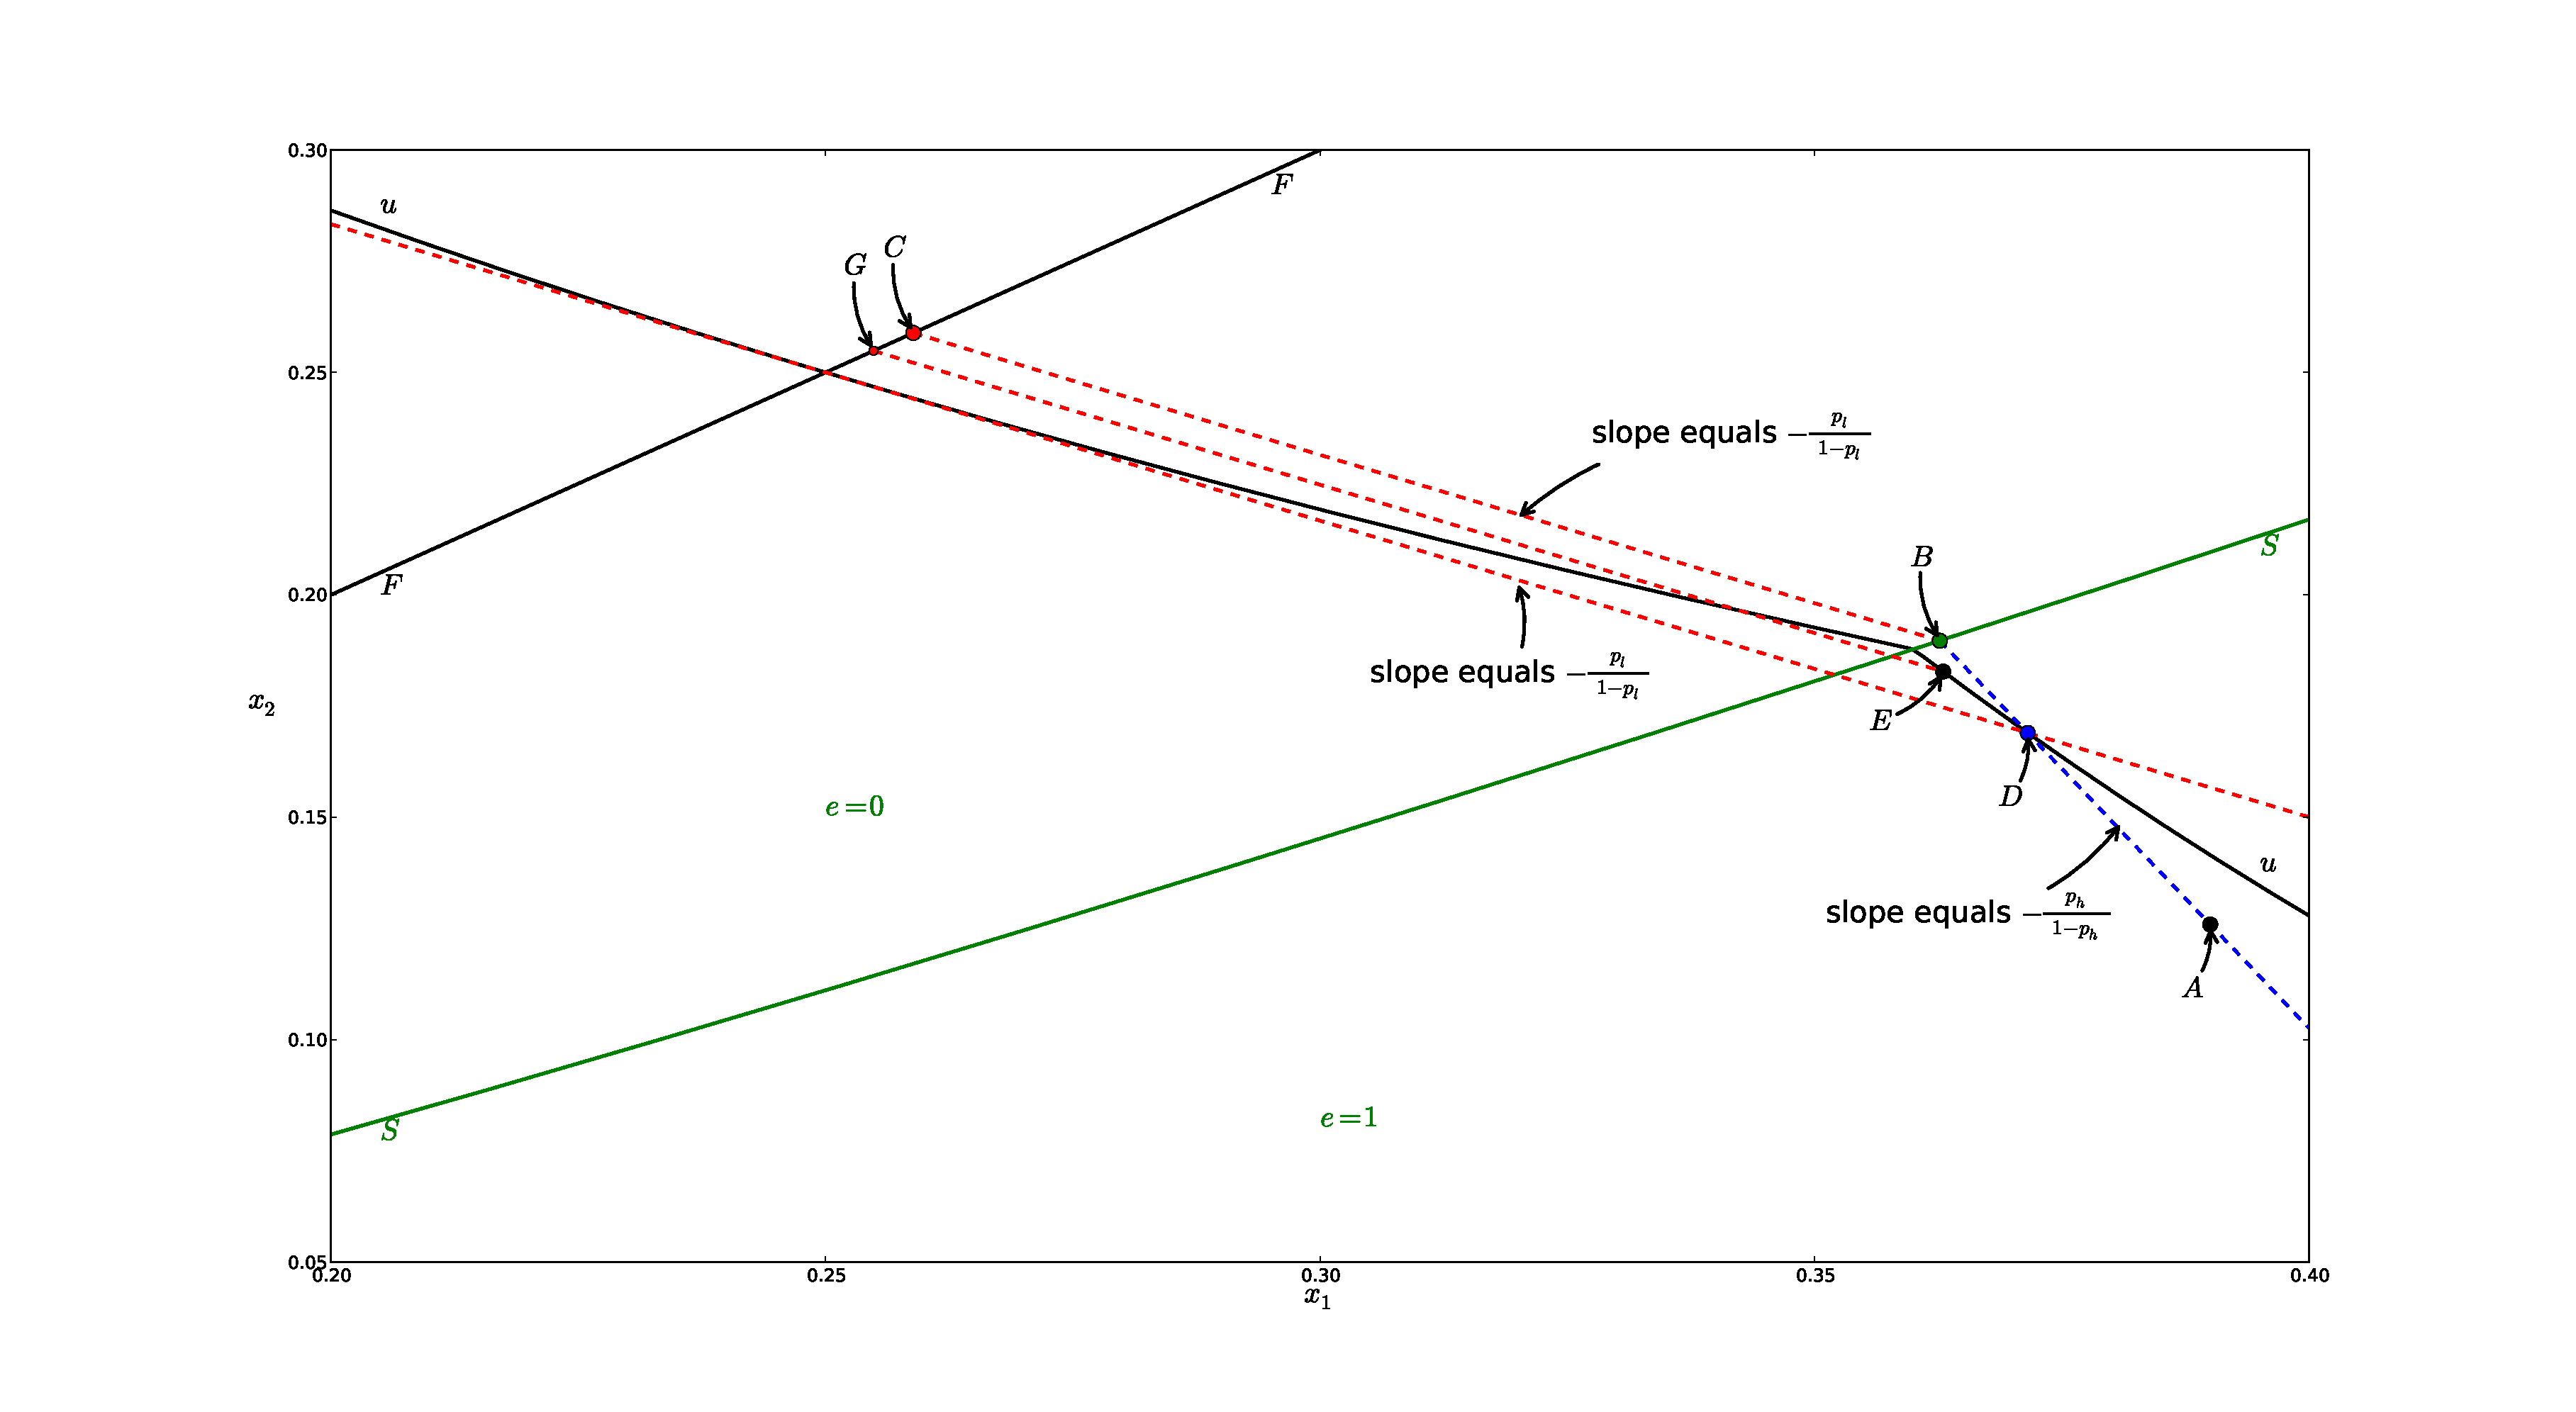
\epsfig{file=KahnMookerjee.eps,height=6cm,width=10cm} \vspace*{0mm}
\caption{First, second and third best contracts.}
\label{fig:insurancecontracts}
\end{figure}
\end{frame}


\begin{frame}[allowframebreaks]\frametitle{Results}
\label{sec-7-4}
\begin{itemize}

\item consider endownment point $A$\\
\label{sec-7-4-1}%
\item if $P$ can commit to exclusive contract, he gets the second best contract $B$\\
\label{sec-7-4-2}%
\item however, $P$ cannot make such a commitment, the insurer that would offer $B$, would make a loss:
\label{sec-7-4-3}%
\begin{itemize}

\item after having signed on for $B$, $P$ would find another insurer who is willing to offer contract $C$\\
\label{sec-7-4-3-1}%
\item $C$ offers full insurance and since it lies on the insurer's isoprofit line with slope $p_{l}/(1-p_{l})$ the second insurer does not make a loss (and $P$ strictly benefits)\\
\label{sec-7-4-3-2}%
\item however, this implies that $P$ chooses $e=0$ making contract $B$ loss making for the first insurer\\
\label{sec-7-4-3-3}%
\item contract $B$ is not offered in equilibrium\\
\label{sec-7-4-3-4}%
\end{itemize} % ends low level

\item the first papers in this literature focused on the following equilibrium: full insurance at inefficiently low effort\\
\label{sec-7-4-4}%
\item to see this, consider endowment point $E$
\label{sec-7-4-5}%
\begin{itemize}

\item equilibrium contract is given by $G$ on insurer's isoprofit line with slope $p_{l}/(1-p_{l})$\\
\label{sec-7-4-5-1}%
\item hence $G$ does not lead to a loss\\
\label{sec-7-4-5-2}%
\item no incentive for $P$ to contract with other insurers\\
\label{sec-7-4-5-3}%
\item the inefficiency here is the low effort level\\
\label{sec-7-4-5-4}%
\end{itemize} % ends low level

\item Kahn and Mookerjee point out that another equilibrium exists\\
\label{sec-7-4-6}%
\item consider again endownment point $A$, then equilibrium contract is given by $D$
\label{sec-7-4-7}%
\begin{itemize}

\item this leads to nonnegative profits as it lies on isoprofit line with slope $p_{h}/(1-p_{h})$ and $e=1$ ($D$ lies below $SS$ curve)\\
\label{sec-7-4-7-1}%
\item consumer has no (strictly positive) incentive to contract with another insurer\\
\label{sec-7-4-7-2}%
\item indifference curve through $D$ lies everywhere above isoprofit line through $D$ with slope $p_{l}/(1-p_{l})$\\
\label{sec-7-4-7-3}%
\item hence no strictly positive surplus can be generated by contracting with further insurers\\
\label{sec-7-4-7-4}%
\item $D$ is third best outcome\\
\label{sec-7-4-7-5}%
\item although $P$ is indifferent to contract to full insurance, such further contracting would break the equilibrium (as insurer offering $D$ would make a loss)\\
\label{sec-7-4-7-6}%
\item hence we use the assumption that $P$ sticks to equilibrium when indifferent\\
\label{sec-7-4-7-7}%
\end{itemize} % ends low level

\item contract $D$ has efficient effort but leads to underinsurance (even less insurance than second best)\\
\label{sec-7-4-8}%
\item hence inability to commit to exclusive contract leads either to ineffient low effort or to underinsurance\\
\label{sec-7-4-9}%
\item note that in equilibrium, $P$ will only contract with one insurer
\label{sec-7-4-10}%
\begin{itemize}

\item hence, if one observes that in reality people only contract with one insurer, this does not mean that exlusive contracts are (costlessly) available\\
\label{sec-7-4-10-1}%
\item further, this does not imply that lack of commitment has no
  effect on equilibrium outcome\\
\end{itemize}
\label{sec-7-4-10-2}%
\item monopoly insurer can offer a more efficient second best contract\\
\label{sec-7-4-10-3}%
\item however, monopolist will also appropriate more of the surplus\\
\label{sec-7-4-10-4}%
\item not clear that monopoly insurer is better for $P$ than competitive insurance market\\
\label{sec-7-4-10-5}%
\end{itemize} % ends low level
\end{frame}



\part[lecture 3]{Offer game and beliefs}

\section{Segal and Whinston (2003)}

\subsection{Hart and Tirole (1990)}

\begin{frame}{Beliefs in offer games}
  \begin{itemize}
  \item HT90 assume passive beliefs: upstream monopolist cannot commit
    to supplying the monopoly output level (in total)
  \item U has an incentive to deviate to higher output level than
    $q^m/2$ with downstream firm
  \item equilibrium output level equals Cournot outcome
  \item \emph{Check} that with symmetric beliefs upstream monopolist can
    implement the monopoly output (without using exclusive contracts)
    [hint: check what happens if upstream firm deviates and offers one
    downstream firm a higher output level (than $q^m/2$)]
  \end{itemize}
\end{frame}


\begin{frame}{Robust predictions}
  \begin{itemize}
  \item HT90 outcome depends on the assumption of (passive) beliefs
  \item Can we come up with predictions independent of beliefs?
  \item SW03: identify properties of equilibrium outcomes that are
    robust in the sense that they must be satisfied by all equilibria
    of all bilateral contracting games
  \item idea is to consider contracting games where parties can offer
    each other a menu-contract from which the principal can then
    choose (rather than a ``point contract'')
  \item Introducing such a menu contract bounds the set of possible outcomes
  \item Only outcomes between the pairwise stable outcome (Cournot)
    and the competitive outcome (price equals marginal costs) can be
    an equilibrium
  \end{itemize}
\end{frame}

\subsection{Model}

\begin{frame}[allowframebreaks]{Model}
  \begin{itemize}
  \item Retailer $i$ has profit: $U_i = P(X)x_i -t_i$ where $P(.)$
    denotes inverse demand as a function of $X= \sum_{i \in N} x_i$
    and $t_i$ denotes transfer from $i$ to manufacturer $M$
  \item In other words, $i$ sells without (further) costs
  \item $M$'s profit: $U_M = \sum_{i \in N} t_i - c(X)$
  \item Assume $c(0)=0,c'(.),c''(.) >0$
  \item define competitive outcome $p^c,X^c$ as
    \begin{itemize}
    \item $\{X^c\} = \arg\max_X p^c X - c(X)$
    \item $p^c = P(X^c)$
    \end{itemize}
  \item we assume that competitive outcome exists and is unique
  \item further assume $p^c X-c(X)$ is strictly decreasing for $X \geq
    X^c$ and $P(X) \leq p^c$ for each $X \geq X^c$
  \item Contracting game: lasts for $K$ periods. In each period $k$, a
    subset $A_k \subset N$ of retailers simultaneously offers menus to $M$ and
    simultaneously $M$ offers menus to $M_k \subset N$ retailers
  \item $M$ and retailers simultaneously decide whether to accept the
    contracts offered to them
  \item Assume $\cup_{k=1}^K (A_k \cup M_k) =N$
  \item $M$ observes entire history, retailer $i$ only observes the
    offers made to him and whether $M$ accepted/rejected his offers to $M$
  \item At the end of the game $M$ chooses $(x_i,t_i)$ from the last
    contract accepted with retailer $i$ and $(0,0)$ if no contract has
    been accepted with $i$
  \item We consider pure-strategy (weak) Perfect Bayesian Equilibrium
    (PBE): FT page 325, Mas-Colell et al. page 285
  \item parties can offer singleton contracts or menus; for reasons
    that become clear below we focus on the competitive menu:
    \begin{equation}
      \label{eq:CompMenuC}
      C = \{ (x,p^c x)|x \in [0,X^c] \}
    \end{equation}
  \item (IR) constraint for retailer $i$: $P(X)x_i - t_i \geq 0$
  \item Define the function $\Pi^c(X_{-i})$ as
    \begin{equation}
      \label{eq:PiCXminusi}
      \Pi^c(X_{-i}) = \begin{cases}
        p^c (X^c-X_{-i})-c(X^c) & \text{if } X_{-i} \leq X^c \\
        -c(X_{-i}) & \text{otherwise}
      \end{cases}
     \end{equation}
  \item Which outcomes can be sustained in equilibrium?
  \end{itemize}
\end{frame}

\subsection{Pairwise stability}

\begin{frame}[allowframebreaks]{Menu deviation condition}
  \begin{proposition} \label{propos:menudeviation}
    In any PBE $(\hat{x},\hat{t})$ it must be the case that for
    each retailer $i \in N$ the following condition holds:
    \begin{equation}
      \label{eq:MenuDeviation}
      \tag{MD} P(\hat{X})\hat{x}_i - c(\hat{X}) \geq \Pi^c(\hat{X}_{-i})
    \end{equation}
  \end{proposition}
  \begin{itemize}
  \item Interpretation: the equilibrium joint profit of $M$ and $i$ is
    higher than the profit they can get if $M$ offers $i$ the
    competitive menu $C$ and then chooses its profit maximizing point
    from $C$ (\emph{check} that RHS corresponds to this choice from $C$)
  \item \textbf{Proof}: Suppose not; i.e. there exists $i \in N$ such that
    \begin{equation} \label{eq:SN}
      P(\hat{X})\hat{x_i} - c(\hat{X}) < \Pi^c(\hat{X}_{-i})
    \end{equation}
  \item let $\bar{k}$ denote the last period in which $M$ and $i$ have
    a contracting opportunity
  \item Suppose that $M$ makes the offer in this period:
    \begin{itemize}
    \item $M$ deviates by only offering $(0,0)$ to $i$ prior to
      $\bar{k}$ and by rejecting all offers from $i$
    \item in period $\bar{k}$, $M$ offers $i$ menu $C$ with $t_i$ that
      is $\ve >0$ below the corresponding competitive transfer: $i$
      makes a positive profit ($\ve$) with this menu and accepts
      (Note: this is the point where normally we have to invoke $i$'s
      beliefs; why are beliefs not relevant here?)
    \item $M$ sticks to equilibrium strategies with other players
      (perhaps $M$ can do even better) and gets payoff:
        \begin{align}
          \sum_{j \neq i} \hat{t}_j + \Pi^c(\hat{X}_{-i}) - \ve &>
          \sum_{j \neq i} \hat{t}_j + P(\hat{X})\hat{x}_i - c(\hat{X})
          \\
          & \geq  \sum_{j \in N} \hat{t}_j - c(\hat{X})
        \end{align}
      \item second inequality follows because in hypothesized
        equilibrium $i$ will not pay more than $P(\hat{X})\hat{x}_i$
    \end{itemize}
  \item Suppose that $i$ makes offer in $\bar{k}$
    \begin{itemize}
    \item $i$ offers $M$ the menu $C$ minus payment
     \begin{equation*}
      \Delta = \Pi^c(\hat{X}_{-i})-(\hat{t}_i-c(\hat{X})) - \ve
     \end{equation*}
    that is, $t_i = p^c(X^c-\hat X_{-i}) - \Delta$
    \item if accepted, the retailer gets
      \begin{equation*}
        p^c(X^c - \hat{X}_{-i}) - t_i = \Delta > P(\hat{X})\hat{x}_i -\hat{t}_i
      \end{equation*}
    \item \emph{check} that the last inequality follows (for $\ve>0$ small
      enough) from the definition of $\Delta$ and equation (\ref{eq:SN})
    \item The principal gains as well because:
      \begin{equation*}
        t_i - c(X^c) > \hat{t}_i - c(\hat{X})
      \end{equation*}
    \item \emph{check} that this is true for $\ve >0$ \qed
    \end{itemize}
  \end{itemize}
\end{frame}

\begin{frame}[allowframebreaks]{Pairwise stability}
  \begin{itemize}
  \item We say that $\hat{x}$ is pairwise stable if
    \begin{equation}
      \label{eq:PairwiseStable}
      \hat{x}_i \in \arg\max_{x} P(x+\hat{X}_{-i})x-c(x+\hat{X}_{-i})
    \end{equation}
    for each $i \in N$
  \item Note that $\hat{X}_{-i}$ is taken as given here: it is as if
    $M$ and $i$ consider their joint surplus where $i$ has passive
    beliefs
  \item Note that pairwise stability is stronger than (MD) because
    (MD) only checks for deviations using menu $C$
  \end{itemize}
  \begin{proposition}
    Any pairwise stable $\hat{x}$ satisfies (MD)
  \end{proposition}
  \begin{itemize}
  \item \textbf{Proof} Suppose not; i.e. $\hat{x}$ is pairwise stable
    but there exists $i$ such that
    \begin{equation*}
      P(\hat{X})\hat{x_i} - c(\hat{X}) < \Pi^c(\hat{X}_{-i})
    \end{equation*}
    then we have that
    \begin{equation*}
      p^c(X^c - \hat{X}_{-i}) - c(X^c) >  P(\hat{X})\hat{x_i} - c(\hat{X})
    \end{equation*}
    or equivalently
    \begin{equation*}
      P(x+ \hat{X}_{-i})x - c(x+ \hat{X}_{-i}) >  P(\hat{X})\hat{x_i} - c(\hat{X})
    \end{equation*}
    for $x=X^c- \hat{X}_{-i}$.
  \item This contradicts that $\hat{x}$ is pairwise stable. \qed
  \end{itemize}
\end{frame}

\subsection{Competitive outcome and competitive menu}

\begin{frame}[allowframebreaks]{Convergence to competitive outcome}
  \begin{proposition}
    If $\{\hat{X}^N \}_{N=1}^{\infty}$ is a sequence of PBE aggregate
    trades in a sequence of bilateral contracting games with $N$
    retailers, then:
    \begin{description}
    \item[(a)] $\hat{X}^N \leq X^c$ for all $N$
    \item[(b)] if $W(X) \equiv P(X)X-c(X)$ is bounded above on $X \in
      \re_+$, then $\hat{X}^N \rightarrow X^c$ as $N \rightarrow \infty$
    \end{description}
  \end{proposition}
  \begin{itemize}
  \item \textbf{Proof.} Suppose --by contradiction-- that (a) does not
    hold; i.e. $\hat{X}^N > X^c$ for some $N$. Because $P(X)$ is
    falling in $X$ for $X>X^c$ we have
    \begin{align}
      P(\hat{X}^N)\hat{x}_i^N - c(\hat{X}^N) & < p^c \hat{x}^N_i - c(\hat{X}^N) \\
      & \leq \max_x p^c x - c(\hat{X}^N_{-i} +x) \\
      & =
      \begin{cases}
        -c(\hat{X}^N_{-i}) & \text{if } \hat{X}^N_{-i} > X^c \\
        p^c(X^c - \hat{X}^N_{-i})-c(X^c) & \text{otherwise}
      \end{cases}
    \end{align}
    which contradicts proposition \ref{propos:menudeviation}.
  \item Part (a) implies that $\hat{X}^N_{-i} \leq \hat{X}^N \leq X^c$
  \item hence we have $\Pi^c(\hat{X}^N_{-i}) = p^c (X^c -
    \hat{X}^N_{-i}) - c(X^c)$.
  \item Adding up (MD) over $i \in N$ we get
    \begin{equation*}
      P(\hat{X}^N)\hat{X}^N-Nc(\hat{X}^N) \geq p^c(NX^c - (N-1)\hat{X}^N)-Nc(X^c)
    \end{equation*}
    or equivalently (\emph{check})
    \begin{align}
      p^c \hat{X}^N-c(\hat{X}^N) & \geq \frac{N}{N-1} (p^c X^c -
      c(X^c)) -\frac{1}{N-1} W(\hat{X}^N) \\
      & \geq \frac{N}{N-1} (p^c X^c -
      c(X^c)) -\frac{1}{N-1} \sup_X W(X) \\
      & \rightarrow p^cX^c - c(X^c) \text{ as } N \rightarrow \infty
    \end{align}
  \item Hence $\hat{X}^N \rightarrow X^c$ as $N\rightarrow \infty$
    because $X^c = argmax_X p^c X -c(X)$ \qed
  \end{itemize}
\end{frame}

\begin{frame}[allowframebreaks]{What is so special about menu $C$?}
  \begin{lemma}
    Consider the set of menus
    $(x_i(X_{-i}),P(x_i(X_{-i})+X_{-i})x_i(X_{-i}))$ where
    $x'_i(X_{-i})$ exists. Out of this set of menus, the profit
    maximizing menu for $M$ is the competitive menu $C$.
  \end{lemma}
    \begin{itemize}
    \item \textbf{Proof.} $M$ chooses the profit maximizing point out of the menu:
      \begin{equation*}
        \Pi_i(X_{-i}) = \max_{t_i,x_i} \{t_i - c(x_i + X_{-i}) \}
      \end{equation*}
      envelope theorem implies (see (IC) in equation (\ref{eq:ICasyminfo}))
      \begin{equation}
        \label{eq:ICmenu}
        \Pi'_i(X_{-i}) = - c'(x_i+X_{-i})
      \end{equation}
    \item We also have
      \begin{equation*}
        \Pi_i(X_{-i}) = x_i(X_{-i})P(x_i(X_{-i})+X_{-i})-c(x_i(X_{-i})+X_{-i})
      \end{equation*}
    \item taking the derivative and setting it equal to equation
      (\ref{eq:ICmenu}) yields
      \begin{multline}
        -c'(x_i(X_{-i})+X_{-i})=x'_i(X_{-i})P(x_i(X_{-i})+X_{-i})+ \\
        (x'_i(X_{-i})+1)(x_i(X_{-i})P'(x_i(X_{-i})+X_{-i})-c'(x_i(X_{-i})+X_{-i}))
      \end{multline}
    \item which is a differential equation for $x_i$ with boundary
      condition $x_i(X^c)=0$
    \item \emph{check:} $x_i(X_{-i}) = X^c - X_{-i}$ solves this differential equation
    \item this solution for $x_i$ is implemented by menu $C$. \qed
    \end{itemize}
\end{frame}

\subsection{Equilibrium trades}

\begin{frame}[allowframebreaks]{Characterization of PBE trades $\hat{x}$}
  \begin{proposition}
    $(\hat{x},\hat{t})$ is a PBE outcome if and only if it
    satisfies (IR) and (MD).
  \end{proposition}


    \begin{itemize}
    \item \textbf{Proof.} Necessity of (MD) follows from proposition
      \ref{propos:menudeviation}. If (IR) is not satisfied, retailers
      will reject the outcome.
    \item For sufficiency we need to verify that $M$ cannot benefit
      from a multilateral deviation to a group $D$ of retailers
    \item Since for each retailer the optimal deviation uses $C$, the
      max. profit $M$ can get from such a deviation equals
      \begin{eqnarray*}
        \Pi_D^C(\hat{X}_{-D}) &=& \max_{(x_D,t_D) \in C^{|D|}} \sum_{i \in
          D} t_i - c(X_D + \hat{X}_{-D}) \\
        &=& p^c (X^c-\hat{X}_{-D}) - c(X^c) \\
        &=& \pi^c - p^c(\hat{X}-\hat{X}_{D})
      \end{eqnarray*}
    \item summing (MD) over $i \in D$ and noting that $\sum_{i \in D}
      X_{-i} = \sum_{i \in D} (X-X_i) = |D|X - X_D$ we get
      \begin{eqnarray*}
   \hspace{-8mm}     P(\hat{X}) \sum_{i \in D} \hat{x}_i - |D| c(\hat{X}) &\geq&
        |D|\pi^c - |D| p^c \hat{X} + p^c \hat{X}_D \\
        &=& \pi^c - p^c(\hat{X}-\hat{X}_D)+(|D|-1)(\pi^c-p^c \hat{X})
      \\
        &\geq&  \pi^c - p^c(\hat{X}-\hat{X}_D)-(|D|-1)c(\hat{X})
      \end{eqnarray*}
      because $\pi^c \geq p^c \hat{X} -c(\hat{X})$.
    \item Hence we find that
      \begin{equation*}
        P(\hat{X})\hat{X}_D - c(\hat{X}) \geq \pi^c -
        p^c(\hat{X}-\hat{X}_D) = \Pi^C_D(\hat{X}_{-D})
      \end{equation*}
    \item In words, (MD) implies that multilateral deviation (to
      contract $C$) is not
      profitable for $M$
    \item A PBE sustaining $(\hat{x},\hat{t})$ takes the following form:
      \begin{itemize}
      \item $M$ offers $(\hat{x}_i,\hat{t}_i)$ to each retailer $i$
      \item retailer $i$ offers $(\hat{x}_i,\hat{t}_i)$ to $M$
      \item retailer $i$ accepts $(\hat{x}_i,\hat{t}_i)$ and any other
        menu that gives $i$ non-negative profits for sure (best such
        menu from $M$'s point of view is the $C$ menu)
      \item Any other offer $(\tilde{x}_i,\tilde{t}_i)$ to $i$ leads
        to beliefs $\tilde{X}_{-i}$ such that
        \begin{equation*}
          P(\tilde{x}_i + \tilde{X}_{-i})\tilde{x}_i -\tilde{t}_i<0
        \end{equation*}
      \item and is rejected. \qed
    \end{itemize}
    \end{itemize}
\end{frame}

\begin{frame}{Conclusions}
  \begin{itemize}
  \item HT90 find that with private offers and passive beliefs the
    Cournot outcome is the equilibrium; monopoly profits cannot be
    sustained in equilibrium
  \item However, passive beliefs are not always convincing and other
    (e.g. symmetric) beliefs lead to other outcomes
  \item SW03 allow parties to offer each other a menu of contracts
    from which $M$ can choose
  \item This narrows down the possible equilibrium outcomes: only
    outcomes between the bilaterally stable one (Cournot) and the
    competitive outcome are robust to the introduction of such menus
    of contracts
  \end{itemize}
\end{frame}
\part[lecture 4]{Bidding games and menu auctions}

\section{Bernheim and Whinston (1986)}

\subsection{Model}

\begin{frame}[allowframebreaks]{Menu auction model}
  \begin{itemize}
  \item Auctioneer $M$ and set of bidders $\Im$
  \item $J$ denotes subset of bidders and $\bar{J}$ is its complement
  \item possible allocations $s \in S$ where $S$ is a finite set
  \item $M$'s cost of implementing $s$ equals $d(s)$
  \item $j$'s utility from $s$ is $g_j(s)$
  \item capital $G$ denotes a sum: $G_J(s) = \sum_{j \in J} g_j(s)$
  \item set of allocations that maximize utility of $J$ bidders and $M$
    \begin{equation}
      \label{eq:SJ}
      S^J = \arg\max_{s \in S} G_J(s)-d(s)
    \end{equation}
  \item $S^*=S^{\Im}$ set of efficient allocations for $M$ and $\Im$ together
  \item each bidder $j$ makes contingent bids $f_j(s) \geq 0$
  \item $M$ implements allocation $s$ that maximizes her utility $u_M(s) =
    \sum_{j \in \Im} f_j(s) - d(s)$.
  \item Set of such allocations:
    \begin{equation}
      \label{eq:Istar}
      I^*(\{f_j\}_{j \in \Im}) = \arg\max_{s \in S} u_M(s)
    \end{equation}
  \item Utility bidder $j$ is denoted $u_j(s) = g_j(s) - f_j(s)$
  \item With sums: $U_J(s) =\sum_{j \in J} u_j(s) = G_J(s) - F_J(s)$
  \item $(\{f_j\}_{j \in \Im},s^0)$ is a \emph{Nash equilibrium} if
    \begin{itemize}
    \item $f_j(s^0) \geq 0$ for all $j \in \Im$ and $s \in S$
    \item $s^0 \in  I^*(\{f_j\}_{j \in \Im})$
    \item No bidder $j$ has a strategy $\tilde{f}_j \geq 0$ that would yield
      higher utility than $u_j(s^0)$
    \end{itemize}
  \end{itemize}
\end{frame}

\subsection{Equilibrium}

\begin{frame}[allowframebreaks]{Nash equilibrium}
\begin{lemma}
      $(\{f_j\}_{j \in \Im},s^0)$ is a \emph{Nash equilibrium} if and
      only if
      \begin{enumerate}
      \item $f_j \geq 0$ for all $j \in \Im$
      \item $s^0 \in  I^*(\{f_j\}_{j \in \Im})$: $s^0$ maximizes $M$'s utility
      \item $g_j(s_0) +F_{-j}(s^0)-d(s^0) \geq g_j(s) +F_{-j}(s)
        -d(s)$ for all $j \in \Im$ and $s \in S$: coalition of $i$ and
        $M$ cannot gain by deviating to $s \neq s^0$
      \item for every $j \in \Im$ there exists $s^j \in  I^*(\{f_j\}_{j
          \in \Im})$ such that $f_j(s^j)=0$
      \end{enumerate}
    \end{lemma}
\begin{itemize}
  \item \textbf{Proof.} \emph{Necessity}
    \begin{enumerate}
    \item by assumption bids must be non-negative
    \item $M$ maximizes payoffs in equilibrium
    \item Suppose not, i.e. there exists $j$ and $\tilde{s}$ such that
      \begin{equation} \label{eq:TildeSj}
        g_j(\tilde{s})-\left([F_{\Im}(s^0)-d(s^0)]-[F_{-j}(\tilde{s})-d(\tilde{s})] \right)
        > g_j(s^0)-f_j(s^0)
      \end{equation}
      then $j$ can deviate to
      \begin{equation*}
        \tilde{f}_j(\tilde{s})=[F_{\Im}(s^0)-d(s^0)]-[F_{-j}(\tilde{s})-d(\tilde{s})]
        + \ve
      \end{equation*}
      for $\ve>0$ sufficiently small. \emph{Check} that $M$ will choose
      $\tilde{s}$ because
      \begin{equation*}
        U_M = \tilde{f}_j(\tilde{s})+F_{-j}(\tilde{s})-d(\tilde{s}) > F_{\Im}(s^0)-d(s^0)
      \end{equation*}
       and \emph{check} that $j$ gains because
      \begin{equation*}
        U_j = g_j(\tilde{s})-\tilde{f}_j(\tilde{s}) > g_j(s^0)-f_j(s^0)
      \end{equation*}
    \item if such $s^j$ does not exist for $j$, $j$ can lower $f_j(s)$
      for each $s \in I^*(\{f_j\}_{j \in \Im})$. This will not change
      $M$'s choice of $s$ but clearly $j$'s payoff increases.
    \end{enumerate}
  \item \emph{Sufficiency} Suppose that $(\{f_j\}_{j \in \Im},s^0)$
    satisfies conditions 1-4 but is not a Nash equilibrium. Then there
    exists bidder $j$ and strategy $\tilde{f}_j$ such that this
    deviating strategy induces $M$ to choose $\tilde{s}$:
    \begin{equation}
      \label{eq:DeviatingTildef}
      \tilde{f}_j(\tilde{s}) +F_{-j}(\tilde{s})-d(\tilde{s}) \geq
      \tilde{f}_j(s)+F_{-j}(s)-d(s) \text{ for all } s \in S
    \end{equation}
    and $j$ strictly gains:
    \begin{equation}
      \label{eq:jGains}
      g_j(\tilde{s})-\tilde{f}_j(\tilde{s}) > g_j(s^0)-f_j(s^0)
    \end{equation}
    Combining this equation with condition 3 yields
    \begin{equation*}
      \tilde{f}_j(\tilde{s})-f_j(s^0) < g_j(\tilde{s})-g_j(s^0) \leq
      F_{-j}(s^0)-F_{-j}(\tilde s) - d(s^0) +d(\tilde s)
    \end{equation*}
    Or equivalently
    \begin{equation*}
      \tilde{f}_j(\tilde{s}) < [F_{\Im}(s^0) - d(s^0)] -[F_{-j}(\tilde s) -d(\tilde s)]
    \end{equation*}
    by condition 4 there exists $s^j$ such that
    \begin{equation*}
      0+F_{-j}(s^j)-d(s^j) = F_{\Im}(s^0) - d(s^0)
    \end{equation*}
    hence we have
    \begin{equation*}
      \tilde{f}_j(\tilde{s}) < [\tilde f_j(s^j)+F_{-j}(s^j)-d(s^j)]  -[F_{-j}(\tilde s) -d(\tilde s)]
    \end{equation*}
    because $\tilde f_j \geq 0$.
    Rewriting we have
    \begin{equation*}
      \tilde{f}_j(\tilde{s}) +F_{-j}(\tilde s) -d(\tilde s) < \tilde f_j(s^j)+F_{-j}(s^j)-d(s^j)
    \end{equation*}
    which contradicts equation (\ref{eq:DeviatingTildef}) for
    $s=s^j$. \qed
  \end{itemize}
\end{frame}

\subsection{Truthful strategies and bidders' payoffs}

\begin{frame}[allowframebreaks]{Truthful strategies}
  \begin{itemize}
  \item $f_j$ is a \emph{truthful strategy} relative to $s^0$ if either
    \begin{itemize}
    \item $g_j(s) - f_j(s) =g_j(s^0)-f_j(s^0)$ or
    \item $g_j(s) - f_j(s) \leq g_j(s^0)-f_j(s^0)$ and $f_j(s)=0$
    \end{itemize}
  \item $(\{f_j\}_{j \in \Im},s^0)$ is a \emph{truthful Nash
      equilibrium} if it is a Nash equilibrium and $\{f_j\}_{j \in
      \Im}$ are truthful strategies relative to $s^0$.
  \item In a truthful equilibrium, each bidder reveals his net
    willingness to pay for $s$ relative to $s^0$
  \item The following result shows that bidders (and we) can restrict
    attention to truthful strategies
  \end{itemize}
  \begin{theorem}
    For any set of offers $\{f_j\}_{j \neq i}$, $i$'s best response
    contains a truthful strategy
  \end{theorem}
  \begin{itemize}
  \item Suppose one of $i$'s optimal responses is $f_i$ and with this
    response $M$ chooses $s^0$. Further, assume that $f_i$ is not
    truthful relative to $s^0$. Define strategy $\tilde f_i$ such that
    $\tilde f_i(s^0) =f_i(s^0)$ and $\tilde f_i$ is truthful relative
    to $s^0$. Two possibilities:
    \begin{itemize}
    \item if $M$ chooses $s^0$ under $\tilde f_i$ as well, $i$ does
      not loose from switching to $\tilde f_i$
    \item if $M$ switches to $\tilde s \neq s^0$, it must be the case
      that $\tilde f_i(\tilde s) > f_i(\tilde s) \geq 0$. But then $i$
      cannot loose from using the truthful strategy $\tilde f_i$ because
      \begin{equation*}
        g_i(\tilde s)-\tilde f_i(\tilde s) = g_i(s^0)-\tilde f_i(s^0)
        = g_i(s^0) -f_i(s^0)
      \end{equation*} \qed
    \end{itemize}
  \end{itemize}
\end{frame}

\begin{frame}[allowframebreaks]{Utilities for bidders}
  \begin{theorem}
    In each truthful Nash equilibrium, $M$ chooses $s^0 \in S^*$. For
    each coalition $J \subset \Im$, bidders payoffs satisfy
    \begin{equation}
      \label{eq:bidderspayoffs}
      \sum_{j \in J} \{ g_j(s^0) - f_j(s^0) \} \leq \sum_{j \in \Im}
      g_j(s^0) -d(s^0) - \max_{s \in S} \{\sum_{j \notin J} g_j(s) - d(s) \}
    \end{equation}
  \end{theorem}
  \begin{itemize}
  \item Equation (\ref{eq:bidderspayoffs}) says that a coalition $J$
    cannot get more than its marginal contribution to the ``grand coalition''
  \item We can also write this as saying that the coalition of $M$ and
    $\Im \setminus J$ cannot gain by deviating (excluding $J$):
    \begin{equation*}
      \sum_{j \notin J} g_i(s^0) + \sum_{j \in J} f_j(s^0) -d(s^0)
      \geq \max_{s \in S} \{ \sum_{j \notin J} g_j(s) -d(s) \}
    \end{equation*}
  \item The intuition why $s^0 \in S^*$ is that in a truthful
    equilibrium $M$ takes the marginal valuations of all bidders into
    account
  \item \textbf{Proof.} First, suppose that $M$'s equilibrium choice
    $s^0 \notin S^*$. Then because strategies are truthful relative to
    $s^0$, we have for $s^* \in S^*$ that
    \begin{equation*}
      f_j(s^*) \geq g_j(s^*) -[g_j(s^0)-f_j(s^0)]
    \end{equation*}
  \item summing over all $j$:
    \begin{equation*}
      F_{\Im}(s^*) \geq G_{\Im}(s^*) - G_{\Im}(s^0) + F_{\Im}(s^0)
    \end{equation*}
  \item Therefore
    \begin{multline}
      F_{\Im}(s^*)-d(s^*) \geq \underset{>0 \text{ because }s^* \in
        S^*\text{ and } s^0 \notin S^*}{\underbrace{[G_{\Im}(s^*)-d(s^*)]-
          [G_{\Im}(s^0)-d(s^0)]}} \\
      + [F_{\Im}(s^0)-d(s^0)] > F_{\Im}(s^0)-d(s^0)
    \end{multline}
  \item which contradicts that $M$ chooses $s^0$ in equilibrium
  \item Now consider equation (\ref{eq:bidderspayoffs}). Using
    equation (\ref{eq:SJ}) and the fact that $M$ chooses $s^0$ in
    equilibrium, we have that
    \begin{equation*}
      F_{\Im}(s^0)-d(s^0) \geq  F_{\Im}(s^{\bar{J}})-d(s^{\bar J})
    \end{equation*}
  \item Therefore
    \begin{align}
      F_{J}(s^0) + F_{\bar J}(s^0) -d(s^0) &\geq  F_{J}(s^{\bar{J}})+
      F_{\bar J}(s^{\bar{J}}) -d(s^{\bar J}) \\
      & \geq F_{\bar J}(s^{\bar{J}}) -d(s^{\bar J}) \\
      & \geq [G_{\bar J}(s^{\bar{J}})-G_{\bar J}(s^{0}) + F_{\bar J}(s^{0})] -d(s^{\bar J})
    \end{align}
  \item where the second line follows from $F_{J}(s^{\bar{J}}) \geq 0$
    and the third from the fact that $f_j$ is truthful relative to $s^0$.
  \item \emph{check} that this implies (\ref{eq:bidderspayoffs}). \qed
  \end{itemize}
\end{frame}

\subsection{Application}

\begin{frame}[allowframebreaks]{Menu auction in HT90}
  \begin{itemize}
  \item Consider the Hart-Tirole game with two retailers and one
    manufacturer $M$
  \item Consider a menu auction in which retailers make offers to
    manufacturer
  \item note that these offers depend on the final allocation: on
    $x_i$ and $x_{-i}$.
  \item Assume demand takes the form $p_i(x_i,x_{-i})$, retailers sell
    without further costs
  \item $M$ produces output at costs $c(x_1+x_2)$
  \item Truthful bids imply that they take the form
    \begin{equation*}
      t_i(x_i,x_{-i}) = p(x_i,x_{-i})x_i - \bar{u}_i
    \end{equation*}
    for some $\bar{u}_i \geq 0$
  \item $M$ solves
    \begin{equation*}
      \max_{x_1,x_2} [p(x_1,x_2)x_1 -\bar u_1] + [p(x_2,x_1)x_2 - \bar u_2]-c(x_1+x_2)
    \end{equation*}
  \item Hence the efficient (monopoly) output levels are chosen
  \item Since the coalition $M$ and $R_2$ can deviate and exclude
    $R_1$ we have
    \begin{equation*}
      [p(x_1,x_2)x_1 -\bar u_1] + p(x_2,x_1)x_2 -c(x_1+x_2) \geq
      \max_{x_2} p(x_2,0)x_2 - c(x_2)
    \end{equation*}
  \item or equivalently
    \begin{equation*}
      \bar u_1 \leq [p(x_1,x_2)x_1 + p(x_2,x_1)x_2 -c(x_1+x_2)] -
      \max_{x_2} p(x_2,0)x_2 - c(x_2)
    \end{equation*}
  \item $R_1$ does not get more than his marginal contribution to the surplus
  \end{itemize}
\end{frame}

\section{Martimort and Stole (2003)}

\subsection{Common agency}

\begin{frame}[allowframebreaks]{Common agency}
  \begin{itemize}
  \item BW86 assume that retailer $i$'s offer can depend on $x_{-i}$
  \item Now we assume that $i$'s offer can only depend on $x_i$
  \item Two retailers (as principals) make offers to common agent $M$:
    bidding game
  \item two types of common agency games:
    \begin{itemize}
    \item \emph{intrinsic}: $M$ either accepts both offers or rejects
      both offers from retailers 1 and 2
    \item \emph{delegated}: $M$ can either accept no, one or both offers
    \end{itemize}
  \item two types of contract:
    \begin{itemize}
    \item singleton contracts with just the equilibrium offer
    \item menu contracts with equilibrium offer and out-of-equilibrium offers
    \end{itemize}
  \end{itemize}
  \begin{table}
    \centering
    \begin{tabularx}{\linewidth}{X|XX}
      & intrinsic & delegated \\ \hline
      singleton & $q = q^c$, $U_M =0$ & one retailer, $q =2q^m$, $U_M >0,U_1=U_2=0$  \\
      menu & $q \in [q^c,q^b]$, $U_M=0$  & propos. 5 in MS03
    \end{tabularx}
    \caption{Summary of results}
    \label{tab:summaryMS03}
  \end{table}
\begin{itemize}
\item Note that in MS03 $q^c$ denotes Cournot output and $q^b$ denotes
  competitive output level
\item With intrinsic common agency:
  \begin{itemize}
  \item singleton contracts lead to Cournot outcome
  \item with extended menu contracts, there are multiple equilibria
    with $q^c$ as lower bound on output
  \item hence it is a bit strange that retailers would use extended
    contracts at all $=>$ MS03 section 5 presents a model with asymmetric
    information about $M$'s efficiency. Then a contract is offered for
    each type of $M$ and extended contracts make sense
  \end{itemize}
\item With delegated common agency and singleton contracts:
  \begin{itemize}
  \item there is no equilibrium in which both retailers serve
    $M$. Under some condition there is an equilibrium in which
    retailers compete rents away to become exclusive retailer of $M$,
    selling the monopoly output.
  \end{itemize}
\item In these lectures we will not cover the case with delegated
  common agency and extended menu of contracts: see proposition 5 in
  the paper
\end{itemize}
\end{frame}

\begin{frame}[allowframebreaks]{Model}
  \begin{itemize}
  \item two retailers sell homogeneous good bought from $M$ at
    transfer $t_i$ and no further costs
  \item inverse demand: $P(Q)$ where $Q=q_1+q_2$ with $P(0)>0,|P'(0)|<+\infty,P'<0,P''\leq0$
  \item $M$ produces at cost $c(Q)$ (we focus on $\theta=1$) with $c(0)=c'(0)=0,c',c'',c'''>0$
  \item Retailer $i$'s profit: $U_i = P(q_i+q_{-i})q_i -t_i$
  \item $M$'s profit: $U_M = t_1+t_2-C(q_1+q_2)$; $M$'s outside option
    equals 0 (zero)
  \item $M$ and $i$ can only contract on $q_i$ not on $q_{-i}$
  \item we consider pure strategy symmetric differentiable (in case of
    menu) equilibria

\newpage

  \item Benchmark \emph{per firm} symmetric output levels:
    \begin{itemize}
    \item competitive: $P(2q^b)=c'(2q^b)$
    \item Cournot: $P(2q^c)+q^cP'(2q^c)=c'(2q^c)$
    \item monopoly: $P(2q^m)+2q^mP'(2q^m)=c'(2q^m)$
    \item \emph{check} that: $0<q^m<q^c<q^b$
    \item we assume that aggregate profits $2q^iP(2q^i) -c(2q^i) \geq
      0$ for $i=m,c,b$
    \end{itemize}
  \end{itemize}
\end{frame}

\subsection{Intrinsic common agency}

\begin{frame}[allowframebreaks]{Intrinsic C.A. with singleton contracts}
  \begin{itemize}
  \item contracts are of the form $(q_i,t_i)$
  \end{itemize}
  \begin{proposition}
    Cournot output $q^c$ is the unique (pure strategy symmetric)
    equilibrium
  \end{proposition}
  \textbf{Proof.}
    \begin{itemize}
    \item consider $R_1$'s problem: $M$'s (IR) constraint is
      \begin{equation}
        \label{eq:IRms03}
        t_1+t_2-c(q_1+q_2) \geq 0
      \end{equation}
    \item no reason to leave rents to $M$, hence $R_1$'s optimization
      problem is
      \begin{equation*}
        \max_{q_1} P(q_1+q_2)q_1 - (c(q_1+q_2)-t_2)
      \end{equation*}
    \item first order condition:
      \begin{equation*}
        P'(q_1+q_2)q_1+P(q_1+q_2)-c'(q_1+q_2) =0
      \end{equation*}
    \item by assumptions above second derivative w.r.t. $q_1$ is negative
    \item symmetric solution is $q_1=q_2=q^c$
    \item this is the same outcome as in the HT90 offer game, but now
      we do not need (passive) beliefs: $R_1$ --as part of the Nash
      equilibrium-- takes $(q_2,t_2)$ as given \qed
    \end{itemize}
\end{frame}

\begin{frame}[allowframebreaks]{Intrinsic C.A. with menus}
  \begin{itemize}
  \item $R_i$ offers $M$ a menu $(q_i,T(q_i))$ and $M$ chooses from
    this menu
  \item in equilibrium $M$ chooses only one combination $(q_i,t_i)$ so
    why are the other (out-of-equilibrium) choices relevant?
  \item Suppose $R_1$ would like to deviate from equilibrium by
    changing $q_1$, which $q_2$ would $M$ choose?
    \begin{equation} \label{eq:q2star}
      q_2^*(q_1) = \arg\max_{q_2} T_2(q_2)-c(q_1+q_2)
    \end{equation}
  \item if ``things are concave'', $q_2^*$ solves
    \begin{equation}
      \label{eq:q2starFOC}
      T'_2(q_2^*(q_1))=c'(q_1+q_2^*(q_1))
    \end{equation}
  \item Hence out of equilibrium choices affect the incentives for the
    other retailer to deviate
  \item Intuitively, if $\dif q^*_2(q_1)/\dif q_1 < 0$ is large in
    absolute value, big incentive for $R_1$ to raise $q_1$
  \item Hence lowest equilibrium output if $q_2$ does not fall at all
    with $q_1$: outcome with singleton contracts
  \item put differently, when $q_2$ hardly increases if $q_1$ falls,
    $R_1$ has big incentive to reduce $q_1$, leads to (relatively) low
    equilibrium output
  \end{itemize}
  \begin{proposition}
    \begin{enumerate}
    \item only $q \in [q^c,q^b]$ can be an equilibrium outcome
    \item each $q \in [q^c,q^b]$ can be an equilibrium outcome
    \end{enumerate}
   In each equilibrium, $M$ gets zero profits: $U_M =0$
  \end{proposition}
    \begin{enumerate}
    \item  \textbf{Proof.} Take $T_2(q_2)$ as given and assume that
      $T_2(q_2)-c(q_1+q_2)$ is concave in $q_2$
      \begin{itemize}
      \item $R_1$ has to take (IR) into account:
        \begin{equation*}
          t_1 +T_2(q^*_2(q_1))-c(q_1+q_2^*(q_1)) \geq 0
        \end{equation*}
      \item no reason to leave rents to $M$, hence $R_1$'s
        optimization problem is to maximize
        \begin{equation*}
          V(q_1) = P(q_1+q_2^*(q_1))q_1 +T_2(q^*_2(q_1))-c(q_1+q_2^*(q_1))
        \end{equation*}
      \item Using envelope argument, first order condition $q_1$ can
        be written as
        \begin{equation}
          \label{eq:FOCq1MS03}
          q_1P'(q_1+q_2^*(q_1)) \left(1+\frac{\dif q_2^*}{\dif q_1}
          \right) + P(q_1+q_2^*(q_1))-c'(q_1+q_2^*(q_1)) =0
        \end{equation}
      \item Use equation (\ref{eq:q2starFOC}) to solve for
        \begin{equation}
          \label{eq:dq2dq1MS03}
          \frac{\dif q_2^*}{\dif q_1} = \frac{c''}{T_2''-c''} \leq 0
        \end{equation}
      \item substitute this into (\ref{eq:FOCq1MS03}) and imposing
        symmetric solution $q_1=q_2=q$ and $T_1(q)=T_2(q)=T(q)$ yields
        \begin{equation}
          \label{eq:solutionq}
          P(2q) + qP'(2q) = c'(2q) - \frac{q P'(2q)c''(2q)}{T''(q)-c''(2q)}
        \end{equation}
      \item $M$ solves
        \begin{equation}
          \label{eq:OptimizationProblemM}
          \max_{q_1,q_2} T(q_1)+T(q_2)-c(q_1+q_2)
        \end{equation}
      \item For this problem to be concave, we need the Hessian to be
        negative semi-definite:
        \begin{gather}
          \label{eq:SOC1} T''(q)-c''(2q) \leq 0 \\
          \label{eq:SOC2} (T''(q)-c''(2q))^2 \geq (c''(2q))^2
        \end{gather}
      \item Substitute (\ref{eq:SOC1}) into (\ref{eq:solutionq}):
        \begin{equation*}
          P(2q)+qP'(2q) \leq c'(2q)
        \end{equation*}
      \item Hence $q \geq q^c$
      \item Now substitute (\ref{eq:SOC2}) into (\ref{eq:solutionq}):
        \begin{equation*}
          P(2q) \geq c'(2q)
        \end{equation*}
      \item Hence $q \leq q^b$
      \item Therefore only $q \in [q^c,q^b]$ can be part of an equilibrium
      \end{itemize}
    \item To show that each $q \in [q^c,q^b]$ can be part of an
      equilibrium, we only need to give an example of a tariff
      function $T(q)$ that gives such a result
      \begin{itemize}
      \item Consider $T(q) = \alpha + \beta q+\hf \gamma q^2$
      \item Then $M$'s first order condition can be written as
        \begin{equation*}
          \beta +\gamma q = c'(2q)
        \end{equation*}
      \item $R_i$'s first order condition (\ref{eq:solutionq}) needs
        to be satisfied:
        \begin{equation} \label{eq:solutionQuadraticT}
          P(2q) + qP'(2q) = c'(2q) - \frac{q P'(2q)c''(2q)}{\gamma-c''(2q)}
        \end{equation}
      \item $M$ gets zero rents:
        \begin{equation*}
          2(\alpha + \beta q+\hf \gamma q^2) = c(2q)
        \end{equation*}
      \item these are three equations in 3 unknowns
        ($\alpha.\beta,\gamma$) that can be solved (see paper for the solution)
      \item $M$'s problem is concave if (\ref{eq:SOC1}) and
        (\ref{eq:SOC2}) hold: is true if and only if $\gamma \leq 0$
      \item ranging from $\gamma=0$ to $\gamma=-\infty$, equation
        (\ref{eq:solutionQuadraticT}) yields $q$ ranging from $q^b$ to $q^c$
      \item \emph{check} for yourself that $R_i$'s optimization problem is
        concave, i.e. $\dif^2 V(q_i)/\dif q_i^2 < 0$ where (from (\ref{eq:dq2dq1MS03})) $\dif
        q_2^*/\dif q_1 = c''/(\gamma-c'')$ \qed
      \end{itemize}
    \end{enumerate}
\end{frame}

\subsection{Delegated common agency}

\begin{frame}[allowframebreaks]{Delegated C.A. with singleton contracts}
  \begin{itemize}
  \item Since $M$ can decide to accept only one contract, $M$ earns a
    positive surplus in equilibrium
  \item In fact, $M$ earns the whole surplus!
  \item retailers cannot offer ``explicit'' exclusive contracts; retailers
    just offer contracts and $M$ decides which to accept
  \item this leads retailers to compete fiercely to get their contract
    accepted by $M$: they compete their surplus away
  \item to make their offer as attractive as possible, they offer a
    contract with the (total) monopoly output
  \item pure strategy symmetric equilibrium only exists if $M$ does
    not want to accept both contracts: condition (\ref{eq:ConditionEq}) below
  \end{itemize}
  \begin{proposition}
    \begin{enumerate}
    \item there is no symmetric pure strategy equilibrium in which $M$ sells to
      both retailers
    \item If
    \begin{equation}
      \label{eq:ConditionEq}
      4q^mP(2q^m)-c(4q^m) < 2q^mP(2q^m)-c(2q^m)
    \end{equation}
    there exists a pure strategy equilibrium in which $M$ sells to
    $R_i$ with probability $\hf$, $M$ produces $2q^m$ receives
    transfer $t_i =2q^mP(q^m)$. Retailers make zero profits and $U_M =
    2q^mP(2q^m)-c(2q^m) >0$
    \end{enumerate}
  \end{proposition}
    \begin{enumerate}
    \item   \textbf{Proof.} Suppose that such a symmetric pure
      strategy equilibrium does exist: $(q,t)$:
      \begin{itemize}
      \item in this (hypothesized) equilibrium, retailers choose $t$
        as low as possible to satisfy
        \begin{eqnarray*}
          U_M& =& 2t-c(2q)  \geq 0 \\
          U_M &\geq & t - c(q)
        \end{eqnarray*}
      \item that is, $M$ should not want to
        \begin{itemize}
        \item either reject both contracts
        \item or reject one contract
        \end{itemize}
      \item the second inequality is binding. Suppose not, i.e. assume
        $2t-c(2q) =0$. Then $t = c(2q)/2 > c(q)$ by convexity of
        $c$. But this implies $U_M = 0 < t-c(q)$ violating the second inequality
      \item With the second inequality binding we find
        \begin{equation}
          \label{eq:tCAdelegated}
          t = c(2q)-c(q)
        \end{equation}
      \item Now suppose $R_1$ offers $q_1 >q$ and $t_1 = c(q_1+q)-c(q)$
      \item then $M$ sells to $R_1$ only because:
        \begin{equation*}
          t_1 - c(q_1) > t_1 + t - c(q_1 +q)
        \end{equation*}
      \item \emph{check} that this follows from equation
        (\ref{eq:tCAdelegated}), $q_1 >q$ and convexity of $c$.
      \item \emph{check} that accepting $R_1$'s contract only is
        better than accepting $R_2$'s contract only
      \item because $M$ sells to $R_1$ only, this deviation to
        $(q_1,t_1)$ is profitable since
        \begin{equation*}
          q_1P(q_1)-(c(q_1+q)-c(q)) > qP(2q)-(c(2q)-c(q))
        \end{equation*}
      \item $q_1 = q+\ve$ for $\ve>0$ small increases the transfer in
        a continuous way, but revenue jumps up for $q>0$.
      \end{itemize}
    \item since $M$ serves at most one retailer, retailers compete to
      become this retailer
      \begin{itemize}
      \item to generate highest surplus, each retailer offers $(2q^m,t)$
      \item with Bertrand competition in $t$ between retailers, each
        retailer offers $t = 2q^m P(2q^m)$
      \item $M$ is indifferent between retailers and randomizes
      \item condition (\ref{eq:ConditionEq}) makes sure that $M$ does
        not accept both contracts
      \item since monopoly profit is assumed to be positive,
        (\ref{eq:ConditionEq}) can only hold if $c$ is ``pretty
        convex'' \qed
      \end{itemize}
    \end{enumerate}
\end{frame}

\subsection{Summary}

\begin{frame}[allowframebreaks]{Conclusion}
  \begin{itemize}
  \item In this lecture we considered two bidding games
  \item hence beliefs play no role in this lecture
  \item in BW86: contract between $M$ and $R_i$ can depend on $(x_i,x_{-i})$
  \item if retailers use truthful strategies, $M$ internalizes
    retailers' marginal valuations between different allocations and
    an efficient outcome is chosen in equilibrium
  \item parties cannot get a payoff higher than their marginal contribution to
    total surplus
  \item MS03: $R_i$'s contract cannot depend on $x_{-i}$
  \item if a retailer can use a menu of contracts, all outcomes
    between pairwise stable and competitive outcome can be sustained
    as equilibrium (same as SW03)
  \item if only singleton contracts can be used, Cournot outcome is equilibrium
  \item with delegated common agency:
    \begin{itemize}
    \item equilibrium implies exclusive dealing (without explicit
      exclusive clauses in the contracts)
    \item $M$ gets strictly positive rent
    \end{itemize}
  \end{itemize}
\end{frame}


\part[lecture 5]{Excusive dealing}


\section{Bernheim and Whinston 1998}

\subsection{Introduction}

\begin{frame}[allowframebreaks]\frametitle{Bernheim and Whinston
    (1998): Motivation}
  \begin{itemize}
  \item Chicago school: the use of exclusionary contracts to foreclose
    entry and hence reduce competition and welfare cannot happen: such
    a contract is not accepted in equilibrium
  \item AB87: $M$ and $R$ can use such a contract to extract rents
    from entrant
  \item RRW91: such a contract is accepted in equilibrium in case of a
    coordination failure among retailers
  \item In both these papers the entrant is passive when $M$ bargains
    with retailers
  \item In BW98,  incumbent $M_a$ and entrant $M_b$ simultaneously
    make offers to retailer $R$
  \item exclusion happens if and only if it is efficient for $M_a,M_b$
    and $R$ jointly
  \item With sequential development of markets over time, it can
    happen that $M_b$ does not enter while this would be efficient for
    $M_a,M_b,R_1$ and $R_2$ jointly
  \item reason is that markets are non-coincident: market 2 (and its
    retailer $R_2$) do not exist yet when $M_a,M_b$ and $R_1$ bargain
  \end{itemize}
\end{frame}

\begin{frame}[allowframebreaks]{Model}
  \begin{itemize}
  \item bidding game: $M_a$ and $M_b$ make offers to $R$
  \item outside option for each player is 0
  \item Notation: (total) exclusive profits $\pi^e_a \geq \pi^e_b >0$
  \item common profits: $0 < \pi^c < \pi^e_a +\pi_b^e$: $M_a$ and $M_b$
    sell partial substitutes
  \item $M_k$ demands net utility $u_k$ for himself ($k=a,b$)
  \item timing of three stage game:
    \begin{itemize}
    \item $M_a$ and $M_b$ simultaneously bid for representation at
      $R$; bid consists of net utility $u_k^e$ for $M_k$ in case of
      exclusive representation and $u_k^c$ for common representation
    \item retailer accepts compatible contracts (or no contract)
    \item aggregate payoffs $\pi_k^l$ materialize $k=a,b;l=c,e$ and
      $R$ pays manufacturer(s) such that their demanded net payoff arises
    \end{itemize}
  \item Hence $R$ receives $u_R = \pi^c-u_a^c-u_b^c$ in case of common
    representation and $u_R = \pi^e-u_k^e$ in case of exclusive deal
    with $M_k$
  \end{itemize}
\end{frame}

\subsection{Results}

\begin{frame}[allowframebreaks]{Exclusive equilibria}
  \begin{itemize}
  \item In exclusive equilibrium we have:
    \begin{itemize}
    \item $u^c_a =u^c_b = +\infty$
      \begin{eqnarray}
        \label{eq:BW98FirstE}
        \pi_a^e -u_a^e = \pi_b^e -u_b^e >0 \\
        \label{eq:BW98SecondE}
        u_a^e \geq 0 \geq u_b^e
      \end{eqnarray}
    \item $R$ accepts offer from $M_a$
    \end{itemize}
  \item To see why this is true, note that
    \begin{itemize}
    \item if $M_a$ sets $u_a^c = +\infty$, $M_b$'s best response is to
      set $u_b^c = +\infty$ as well; hence exclusive equilibrium
      always exists
    \item if $\pi_a^e - u_a^e <0$, $R$ should reject the offer
    \item if $\pi_a^e - u_a^e =0$, $M_b$ can offer $u_b^e < \pi_b^e$
      and win the contract
    \item if $\pi_a^e - u_a^e < \pi_b^e -u_b^e $, $R$ should accept
      $M_b$'s offer
    \item if $\pi_a^e - u_a^e > \pi_b^e -u_b^e $, $M_a$ can raise $u_a^e$
    \item if $u_a^e <0$, $M_a$ should withdraw offer
    \item if $u_b^e >0$, $M_b$ should reduce $u_b^e$ slightly and win
      because of (\ref{eq:BW98FirstE})
    \end{itemize}
  \item There are multiple equilibria: best equilibrium for coalition
    $M_a,M_b$ (making the offers) is $u^e_b=0,u_a^e=\pi_a^e-\pi_b^e$
    and $u_R = \pi^e_b$. $M_a$ gets its contribution to total surplus
  \item if $\pi_a^e > \pi_b^e$ there also exist equilibria with $u_b^e
    <0$ and $u_a^e < \pi_a^e-\pi_b^e$ but these are Pareto dominated
    for $M_a$ and $M_b$ by equilibrium with $u_b^e =0$
  \end{itemize}
\end{frame}

\begin{frame}[allowframebreaks]{Common equilibria}
  \begin{itemize}
  \item If $R$ serves both $M_a$ and $M_b$ we must have
    \begin{equation}
      \label{eq:BW98FirstC}
      \pi^e_a-u_a^e=\pi^e_b-u_b^e=\pi^c-u_a^c-u_b^c >0
    \end{equation}
    and
    \begin{eqnarray}
      \label{eq:BW98SecondC}
      u_k^c \geq 0 \\
      \label{eq:BW98ThirdC}
      u_k^e \leq u_k^c
    \end{eqnarray}
    for $k=a,b$
  \item To see why this is true, note that
    \begin{itemize}
    \item if $\pi^c-u_a^c-u_b^c <0$, $R$ should reject the offer
    \item if $\pi^c-u_a^c-u_b^c =0$ then $\pi_a^e+\pi_b^e -
      u_a^c-u_b^c >0$, hence there is $M_k$ such that
      $\pi_k^e-u_k^c>0$; suppose $k$ deviates by offering
      $\tilde{u}_k^e = u_k^c+\ve$ with $\ve>0$. If $R$ accepts the
      deviating offer, $M_k$ clearly gains. By accepting, $R$ earns
      \begin{equation*}
        \pi_k^e-\tilde{u}_k^e = \pi_k^e-u_k^c-\ve > 0 = \pi^c-u_a^c-u_b^c
      \end{equation*}
      for $\ve>0$ small enough. Hence $R$ accepts the deviating offer
    \item if $\pi^e_k-u_k^e> \pi^c-u_a^c-u_b^c$, $R$ should have
      accepted $M_k$'s exclusive offer
    \item if $\pi^e_k-u_k^e< \pi^c-u_a^c-u_b^c$, $M_{-k}$ can
      profitably deviate by slightly increasing $u_{-k}^c$ and setting
      $u_{-k}^e =+\infty$
    \item if $u_k^c <0$, $M_k$ should withdraw his offer
    \item if $u_k^e > u_k^c \geq 0$, $M_k$ should reduce $u_k^e$
      slightly and win exclusive contract because of (\ref{eq:BW98FirstC})
    \end{itemize}
  \item common equilibrium exists if and only if $\pi^c \geq
    \pi_a^e$. Two ways to see this:
    \begin{itemize}
    \item Write equation (\ref{eq:BW98FirstC}) as
      \begin{equation*}
        \pi^c = \pi_a^e + [u_a^c-u_a^e] + u_b^c \geq \pi_a^e
      \end{equation*}
      because $u_a^c \geq u_a^e$ and $u_b^c \geq 0$
    \item suppose $\pi^c < \pi_a^e$, coalition $R$ and $M_a$ can
      deviate from common outcome and earn $\pi_a^e > \pi^c -u_b^c$
    \end{itemize}
  \item multiple common equilibria: the lower $u_a^e,u_b^e$ the worse
    the equilibrium is for $M_a,M_b$; in the light of
    (\ref{eq:BW98ThirdC}), the best manufacturers can do is to
    set $u_k^e=u_k^c=u_k$
    \begin{itemize}
    \item to see this, suppose $M_k$ chooses $u_k^e < u_k^c$
    \item Then equation (\ref{eq:BW98FirstC}) becomes
      \begin{equation*}
        \pi_k^e-u_k^c < \pi_k^e-u_k^e =\pi^c -u_k^c-u_{-k}^c
      \end{equation*}
    \item hence $u_{-k}^c < \pi^c-\pi^e_k$ while actually both
      manufacturers can get $u_{k}^c = \pi^c-\pi^e_{-k}$ (see below);
      hence the coalition of $M_a,M_b$ is better off by setting  $u_k^e=u_k^c$
    \end{itemize}
  \item with $u_k^c=u_k^e=u_k$ we solve two equations in two unknowns:
    \begin{equation*}
      \begin{cases}
        \pi_a^e -u_a &= \pi^c -u_a-u_b \\
        \pi_b^e -u_b &= \pi^c -u_a-u_b
      \end{cases}
    \end{equation*}
    solution is given by
    \begin{eqnarray*}
      u_a &=& \pi^c-\pi^e_b \\
      u_b &=& \pi^c -\pi^e_a
    \end{eqnarray*}
    each manufacturer gets marginal contribution to surplus $\pi^c$
  \item $R$ earns
    \begin{equation}
      \label{eq:BW98uR}
      u_R = \pi^c -u_a-u_b = \pi_a^e +\pi_b^e - \pi^c >0
    \end{equation}
  \end{itemize}
\end{frame}

\begin{frame}[allowframebreaks]{Common vs Exclusive: three cases}
  \begin{enumerate}
  \item if $\pi^c < \pi_a^e$, there only exists an exclusive
    equilibrium with $M_a$, payoffs are
    \begin{align}
      u_a^e &= \pi_a^e-\pi_b^e \\
      u_b^e &= 0 \\
      u^e_R &= \pi_b^e
    \end{align}
  \item if $\pi^c > \pi_a^e$ then
    \begin{itemize}
    \item exclusive equilibrium above still exists
    \item common equilibrium exists as well, payoffs:
      \begin{align}
        u_a^c &= \pi^c-\pi_b^e > \pi_a^e -\pi_b^e = u_a^e \\
        u_b^c &= \pi^c-\pi_a^e > 0 = u_b^e \\
        u_R^c &= \pi_a^e +\pi_b^e - \pi^c < \pi_b^e = u_R^e
      \end{align}
      because $\pi^c > \pi_a^e$
    \item hence $M_a,M_b$ are better off in common outcome while $R$
      is better off in exclusive outcome. However, $M_a,M_b$ make the
      offers and hence should be able to coordinate on their preferred outcome
    \end{itemize}
  \item if $\pi^c=\pi_a^e$, there is a unique Pareto dominant payoff
    vector (for $M_a,M_b$) which can be achieved through either
    exclusive or common representation
  \end{enumerate}
\end{frame}

\begin{frame}[allowframebreaks]{Two principles}
  \begin{enumerate}
  \item $M_a,M_b$ by choosing the form of representation that is most
    profitable for them, maximize the joint surplus of $M_a,M_b$ and $R$
  \item Exclusion can only happen if there are contracting externalities
    \begin{itemize}
    \item let $\bar{\pi}^c$ denote the joint profit when $M_a,M_b$ fully
      cooperate
    \item $\bar{\pi}^c \geq \pi_a^e$ when $M_a,M_b$ cooperate, they
      can always replicate the exclusive outcome
    \item Hence $\pi^e_a>\pi^c$ and exclusion can only happen if
      $\bar{\pi}^c > \pi^c$: there are contracting externalities, e.g.
      \begin{itemize}
      \item HT90 type of problem on the supply side: input suppliers
        of $M_a,M_b$ produce with costs $C(x_a+x_b)$ with $C',C''>0$
      \item incentive contracts provided by $M_a,M_b$ for a risk
        averse $R$: section V in the paper
      \end{itemize}
    \end{itemize}
  \end{enumerate}
\end{frame}

\begin{frame}[allowframebreaks]{Non-coincident markets}
  \begin{itemize}
  \item two retail markets develop sequentially over time:
    \begin{itemize}
    \item first period/market $M_a,M_b$ and $R_1$ bargain
    \item second period/market $M_a,M_b$ and $R_2$ bargain
    \end{itemize}
  \item $M_a$ is incumbent and $M_b$ is entrant who needs to cover
    entry cost $f>0$
  \item entry by $M_b$ is only profitable if $M_b$ can serve both
    $R_1$ and $R_2$
  \item in the first period, $M_a,M_b$ cannot bargain with $R_2$
    because this market does not exist yet
  \item for each market $t$:
    \begin{itemize}
    \item $x_{ta}^*,x_{tb}^*$ solve
      \begin{equation*}
        \pi^c_t = \bar{\pi}^c_t = \max_{x_a,x_b} \{ R_t(x_a,x_b)-c_a
        x_a -c_b x_b \}
      \end{equation*}
    \item $x_{tk}^e$ solves
      \begin{equation*}
        \pi_{tk}^e = \max_{x_k} \{ R_t(x_k,0)-c_k x_k \}
      \end{equation*}
    \item with $\pi_{ta}^e + \pi_{tb}^e > \pi_t^c$
    \item hence if markets would be completely separate, common
      outcome prevails because $\pi^c_t = \bar{\pi}_t^c \geq \pi_{tk}^e$
    \end{itemize}
  \item Three assumptions:
    \begin{description}
    \item[C1] $0<\pi_2^c-\pi_{2a}^e<f$: if $M_b$ only sells to $R_2$,
      $M_2$'s contribution to total profits does not cover entry cost $f$
    \item[C2] $\pi_1^c-\pi_{1a}^e + \pi_2^c -\pi_{2a}^e >f$: $M_2$'s
      contribution to total profits on both markets does cover $f$:
      aggregate profits (for $R_{1,2},M_{a,b}$) maximized if $M_b$ enters
    \item[C3] $\pi_{1a}^e+\pi_{2a}^e > \pi_1^c + [\pi_2^c-\pi_{2a}^e]
      + [\pi_2^c -\pi_{2b}^e] -f$: profits of $M_a,M_b$ and $R_1$
      higher if $M_b$ does not enter
    \end{description}
  \end{itemize}
  \begin{proposition}
    If (C3) holds, all undominated equilibria involve effective
    exclusion of $M_b$ from market 1 (and hence from market 2)
  \end{proposition}
  \begin{itemize}
  \item \textbf{Proof.} If $M_b$ enters, $M_a,M_b$ and $R_1$ get joint profit
    \begin{equation*}
      \pi_1^c + [\pi_2^c-\pi_{2a}^e] + [\pi_2^c -\pi_{2b}^e] -f
    \end{equation*}
  \item if $M_b$ does not enter, their joint profit is
    \begin{equation*}
       \pi_{1a}^e+\pi_{2a}^e
    \end{equation*}
  \item by (C3) the latter exceeds the former. \qed
  \item by excluding $M_b$, the bargaining power of $M_a$ is increased
    vs $R_2$ which maximizes the joint profit of $M_a,M_b$ and $R_1$
  \end{itemize}
\end{frame}

\begin{frame}[allowframebreaks]{Explicit exclusion clauses}
  \begin{itemize}
  \item In an exclusive outcome, do $M_a$ and $R_1$ need an explicit
    exclusionary clause in their contract?
  \item In other words, once the contract between $M_a$ and $R_1$ is
    signed, do $M_b$ and $R_1$ have an incentive to deviate (if there
    is no such clause)?
  \item joint profit of $M_b$ and $R_1$ is higher if they stick to the
    agreement than if they deviate if and only if
    \begin{equation}
      \label{eq:BW98deviation}
      R_1(x_{1a}^e,0) \geq R_1(x_{1a}^e,x_{1b})-c_b x_{1b} + [\pi_2^c
      -\pi_{2a}^e -f] \text{ for all } x_{1b} > 0
    \end{equation}
  \item if (\ref{eq:BW98deviation}) does hold, $M_a$ and $R_1$ have
    effective exclusion without an explicit clause in their contract
  \item if (\ref{eq:BW98deviation}) does not hold, $M_a$ and $R_1$
    need an explicit exclusionary clause in their contract
  \item if (\ref{eq:BW98deviation}) does not hold, and explicit
    exclusionary clauses are forbidden by law, does his imply the
    common outcome?
  \item Not if the following inequality holds:
    \begin{equation*}
      \max_{x_{a1}^e \text{ s.t } (\ref{eq:BW98deviation})}
      \{R_1(x_{a1}^e,0)-c_a x_{a1}^e \} + \pi_{2a}^e > \pi_1^c +
      [\pi_2^c -\pi_{2b}^e] + [\pi_2^c-\pi_{2a}^e] - f
    \end{equation*}
  \end{itemize}
\end{frame}


\subsection{Conclusions}

\begin{frame}[allowframebreaks]{Summary}
  \begin{itemize}
  \item BW98: bidding game; no beliefs
  \item manufacturers choosing the form of representation that
    maximizes their profits, maximize joint surplus
  \item exclusion can only happen if there are contracting
    externalities such that common (total) profits are below common
    profits that cooperating manufacturers could achieve
  \item with non-coincident markets exclusion can be profitable for
    all parties in the first market because it raises their bargaining
    power in the second market
  \end{itemize}
\end{frame}



\part[lecture 6]{Details of the bargaining environment}

\section{Introduction}

\begin{frame}[allowframebreaks]{Motivation}
  \begin{itemize}
  \item We consider the case with one upstream $M$ and $N$ downstream
    retailers $R_i$ where $M$ makes the offers (offer game)
  \item What is the effect of public offers vs private offers?
  \item In HT90 private offers lead to inefficiently high output and
    public offers lead to an efficient outcome
  \item in Katz and Shapiro (1986a,b) and Kahn and Mookerjee (1998)
    there are public offers and too much trade
  \item in Grossman and Hart (1980) there is a trader with public
    offers and too little trade
  \item what is causing these differences?
  \item How do externalities when trading differ from externalities
    when retailers do not trade?
  \item what is the effect if the manufacturer cannot discriminate in
    its offers to retailers?
  \item what happens if $M$ wants to have unique implementation (like
    in Winter (2004))?
  \end{itemize}
\end{frame}

\section{Segal (1999)}

\subsection{Public offers with discrimination and simple
  implementation}

\begin{frame}[allowframebreaks]{Inefficiency due to externality on non-trader}
  \begin{itemize}
  \item $M$'s trade with $R_i$ is denoted $x_i$; vector of such trades $x$
  \item $X=\sum_{i \in N} x_i$ and $X_{-i} = \sum_{j \neq i} x_j$
  \item $R_i$'s payoff: $u_i(x)-t_i$; usually $u_i(x)= p(X)x_i$
  \item $M$'s payoffs: $u_m(x) = \sum_{i \in N} t_i -c(X)$
  \item default (``no trade'') point: $x_i=0$; $R_i$'s payoff: $u_i(0,x_{-i})$
  \item In HT90 $u_i(0,x_{-i})=0$: if retailer does not buy from $M$,
    he does not produce
  \item In Katz and Shapiro (1986a) profit of firm that does not buy
    license depends on how many firms do buy a license: $L(k)$ with
    $L'(k) \leq 0$.
  \item set of efficient trades:
    \begin{equation}
      \label{eq:S99EfficientTrades}
      \xi^* = \arg\max_x \sum_{i \in N} u_i(x)-c(X)
    \end{equation}
  \item Two-stage game:
    \begin{enumerate}
    \item $M$ commits to set $\{(x_i,t_i)\}_{i \in N}$ of publicly
      observable bilateral contract offers to retailers
    \item retailers simultaneously decide whether to accept or reject
      their resp. offers
    \end{enumerate}
  \item IR-constraints for retailers:
    \begin{equation}
      \label{eq:S99IR}
      u_i(x)-t_i \geq u_i(0,x_{-i})
    \end{equation}
    for all $i \in N$
  \item As there is no reason for $M$ to leave rents to retailers, we can
    solve for $t_i$
  \item $M$'s set of profit maximizing trades:
    \begin{equation}
      \label{eq:S99ProfitTrades}
      \xi^{pu} = \arg\max_x \sum_{i \in N} [u_i(x)-u_i(0,x_{-i})] -c(X)
    \end{equation}
  \end{itemize}
  \begin{proposition}
    If $u_i(0,x_{-i})$ does not depend on $x_{-i}$ for all $i$, then
    $\xi^* =\xi^{pu}$.
  \end{proposition}
  \begin{itemize}
  \item in this case the optimization problems
    (\ref{eq:S99EfficientTrades}) and (\ref{eq:S99ProfitTrades}) coincide.
  \item when externalities on non-traders are absent and $M$ commits
    to compensate retailers for externalities imposed upon them, $M$
    internalizes the externalities and implements efficient trades
  \item This explains why HT90 find an efficient outcome with public contracts
  \item if we do get an inefficient outcome, in which direction does
    it go?
  \item Define
    \begin{align}
      \Xi^* &= \{ \sum_i x_i |x \in \xi^* \} \\
      \Xi^{pu} &= \{ \sum_i x_i |x \in \xi^{pu} \}
    \end{align}
  \end{itemize}
  \begin{proposition} \label{propos:S99PuVsStar}
    With negative externalities on non-traders ($\dif
    u_i(0,x_{-i})/\dif x_j <0$ for $j \neq i$), we find $\Xi^{pu} \geq \Xi^*$.
  \end{proposition}
  \begin{itemize}
  \item \textbf{Proof.} Define the following functions
    \begin{align}
      \label{eq:S99W}
      W(X) &= P(X)X-c(X) \\
      \label{eq:S99R}
      R(X) &= \min_x \{\sum_i u_i(0,x_{-i}) | \sum_i x_i = X \}
    \end{align}
  \item Then $R$ is non-increasing in $X$:
    \begin{itemize}
    \item consider $X,X'$ with $X' \geq X$
    \item take $x$ such that $\sum_i x_i = X$ and $R(X) = \sum_i u_i(0,x_{-i})$
    \item then there exists $x'$ such that $x'_i \geq x_i$ for all $i
      \in N$ and $\sum_i x'_i =X'$
    \item because of negative externalities on non-traders, we have
      \begin{equation*}
        u_i(0,x_{-i}) \geq u_i(0,x'_{-i})
      \end{equation*}
      and therefore
      \begin{equation*}
        R(X') \leq \sum_i u_i(0,x'_{-i}) \leq \sum_i u_i(0,x_{-i}) = R(X)
      \end{equation*}
    \item to simplify, assume that $W$ and $R$ are differentiable and
      compare the first order conditions for the optimization problems
      $\max_X W(X)$ and $\max_X W(X)-R(X)$:
      \begin{eqnarray*}
        W'(X^*) &=& 0 \\
        W'(X^{pu}) &=& R'(X^{pu}) \leq 0
      \end{eqnarray*}
    \item hence $\Xi^* \leq \Xi^{pu}$. \qed
    \item Hence with negative externalities on non-traders we get
      ``overproduction'': $M$ sells more than the monopoly output
      level in order to worsen retailers' outside option
    \item In Katz and Shapiro (1986a) there is a negative externality
      of a trader (downstream firm that buys license) on a non-trader
      (firm that works with old technology); hence R\&D lab tends to
      sell too many licenses
    \item In Katz and Shapiro (1986b) there is a negative externality
      of people that buy sponsored technology $B$ on people that use
      non-sponsored technology $A$; firm $B$ induces too many people (at
      $t=1$) to buy its technology; hence $B$ survives although it is
      inferior to $A$
    \item in Grossman and Hart (1980) there is positive externality of
      shareholders tendering to raider on shareholders that do not
      tender and hence there is too little trade (proposition
      \ref{propos:S99PuVsStar} with positive externalities on non-traders)
    \end{itemize}
  \end{itemize}
\end{frame}

\subsection{Private offers with discrimination and simple implementation}

\begin{frame}[allowframebreaks]{Private offers: externality on
    efficient traders}
  \begin{itemize}
  \item similar two-stage game as above, but now $M$ makes private
    offer to each $R_i$
  \item In other words, $M$ cannot commit to abstain from
    renegotiation with $R_i$ after other retailers have accepted their
    contract
  \item We assume that retailers have passive beliefs: if $\hat{x}$ is
    the equilibrium trade and $R_i$ receives a deviating offer, he
    still beliefs the other retailers were offered $\hat{x}_{-i}$
  \item Hence the IR constraint can now be written as
    \begin{equation}
      \label{eq:S99IRprivate}
      u_i(x_i,\hat{x}_{-i}) - t_i \geq u_i(0,\hat{x}_{-i})
    \end{equation}
  \item As above we can solve for $t_i$:
    \begin{equation*}
      t_i = u_i(x_i,\hat{x}_{-i})-u_i(0,\hat{x}_{-i})
    \end{equation*}
  \item Note that when making offers $x_i$ to retailers, $M$ takes
    $\hat{x}_{-i}$ as given
  \item Hence $\hat{x}$ is an equilibrium trade if and only if
    \begin{equation}
      \label{eq:S99EquilxPrivate}
      \hat{x} \in \arg \max_x \sum_i u_i(x_i,\hat{x}_{-i}) -c(X)
    \end{equation}
  \item let $\xi^{pr}$ denote the set of $\hat{x}$ that satisfy
    equation (\ref{eq:S99EquilxPrivate})
  \end{itemize}
  \begin{proposition}
    If there exists $x^* \in \xi^*$ such that $u_i(x_i^*,x_{-i})$ does
    not depend on $x_{-i}$ for all $i \in N$, then $\xi^{pr} \subset \xi^*$
  \end{proposition}
  \begin{itemize}
  \item \textbf{Proof.} For any $x^{pr} \in \xi^{pr}$ equation
    (\ref{eq:S99EquilxPrivate}) implies that
    \begin{equation*}
      \sum_i u_i(x^{pr})-c(X^{pr}) \geq  \sum_i
      u_i(x_i^*,x_{-i}^{pr})-c(X^*) =  \sum_i u_i(x^{*})-c(X^{*})
    \end{equation*}
    and hence $x^{pr} \in \xi^*$. \qed
  \item To see which way the direction of the distortion goes, define:
    \begin{itemize}
    \item externalities on efficient traders are negative if for all
      $x^* \in \xi^*$ and each $i \in N$, $u_i(x_i^*,x_{-i})$ is
      non-increasing in $x_{-i}$. This is true if $u_i(x_i,x_{-i})=p(X)x_i$.
    \item $\Xi^{pr} = \{ \sum_i x_i | x \in \xi^{pr} \}$
    \end{itemize}
  \end{itemize}
  \begin{proposition}
    Assume $u_i(x_i,x_{-i})=p(X)x_i$. Then $\Xi^{pr} \geq \Xi^*$
  \end{proposition}
  \begin{itemize}
  \item \textbf{Proof.} First order condition for $x^{pr} \in
    \xi^{pr}$ can be written as
    \begin{equation*}
      \frac{\dif u_i}{\dif x_i}(x_i^{pr},x_{-i}^{pr}) - c'(X^{pr}) =0
    \end{equation*}
  \item FOC for $x^* \in \xi^*$:
    \begin{equation*}
      \frac{\dif u_i}{\dif x_i}(x_i^{*},x_{-i}^{*}) - c'(X^{*}) =
      -\sum_{j \neq i} \frac{\dif u_j}{\dif x_i}(x_j^{*},x_{-j}^{*}) \geq 0
    \end{equation*}
  \item hence we find $X^* \leq X^{pr}$. \qed
  \end{itemize}
\end{frame}

\begin{frame}[allowframebreaks]{Comparing public and private offers}
  \begin{itemize}
  \item Assume $u(x_i,x_{-i})=p(X)x_i$ and $u(0,x_{-i})=u_0(X_{-i})$
  \end{itemize}
  \begin{proposition}
    If $p'(X)X< n u'_0(X_{-i})$ for each $X$, then $X^{pu} < X^{pr}$.
  \end{proposition}
  \begin{itemize}
  \item \textbf{Proof.} \emph{Check} that first order conditions for
    $x_i^{pr},x_i^{pu}$ can be written as resp.
    \begin{eqnarray*}
      p'(X^{pr})X^{pr}+p(X^{pr})-c'(X^{pr}) = p'(X^{pr})X^{pr}_{-i} \\
      p'(X^{pu})X^{pu}+p(X^{pu})-c'(X^{pu}) = (n-1) u'_0(X_{-i})
    \end{eqnarray*}
  \item by writing the RHS of the first equation as
    $(n-1)p'(X^{pr})X^{pr}/n$, the result follows. \qed
  \end{itemize}
\end{frame}

\section{Segal (2003a)}

\subsection{Introduction and model}

\begin{frame}[allowframebreaks]{Overview}
  \begin{itemize}
  \item S99 considers private vs public offers
  \item here we only consider public offers
  \item as above, contract with $i$ cannot depend on the choice made
    by $j \neq i$
  \item we consider the cases where $M$ can and cannot discriminate
    between retailers
  \item if $M$ cannot discriminate, she has to offer each retailer the
    same contract
  \item further, we compare the difference between simple and unique implementation
  \item In S99 we considered the case where $M$ can \emph{d}iscriminate and
    only looked at \emph{s}imple implementation. We denote the set of
    outcomes defined in equation (\ref{eq:S99ProfitTrades}) now by $\xi_d^s$
  \item below we will characterize the sets $\xi_n^s$ and $\xi_d^u$
  \item section 4.1.2 in the paper characterizes $\xi_n^u$
  \item characterizing $\xi_d^u,\xi_n^u$ turns out to be
    straightforward for the case of decreasing externalities (see below)
  \end{itemize}
\end{frame}

\begin{frame}[allowframebreaks]{Model}
  \begin{itemize}
  \item $u_i(x_i,x_{-i})=p(x_i + X_{-i})x_i$
  \item hence we focus on negative externalities: $\dif u_i/\dif x_j =
    p'(X)x_i <0$ for each $j \neq i$
  \item externalities can be either
    \begin{itemize}
    \item strictly increasing: $\dif^2 u_i/\dif x_i \dif x_j = p''(X)x_i +p'(X)
      >0$ or
    \item strictly decreasing:$\dif^2 u_i/\dif x_i \dif x_j = p''(X)x_i +p'(X)
      <0$
    \end{itemize}
  \item as above $\Xi^* = \arg\max_X P(X)X-c(X)$
  \item proposition \ref{propos:S99PuVsStar} above: with negative
    externalities at $(0,\ldots,0)$ we have $\Xi^* \leq \Xi^s_d$
  \end{itemize}
\end{frame}

\subsection{Public offers with non-discrimination and simple implementation}

\begin{frame}[allowframebreaks]{Non-discrimination and simple implementation}
  \begin{itemize}
  \item $M$ offers the same menu of contracts to all retailers:
    \begin{equation}
      \label{eq:S03aMenuS}
      S=\{(0,0)\} \cup \{(x_i,t_i)|i \in N\}
    \end{equation}
    where $R_i$ is supposed to choose $(x_i,t_i)$
  \item in equilibrium:
    \begin{itemize}
    \item no $R_i$ prefers (0,0) above $(x_i,t_i)$:
      \begin{equation}
        \tag{$IR_i$}
        u(x_i,X_{-i})-t_i \geq u(0,X_{-i})
      \end{equation}
    \item $R_i$ prefers $(x_i,t_i)$ above $(x_j,t_j)$ for $j \neq i$:
      \begin{equation}
        \tag{$IC_{ij}$}
        u(x_i,X_{-i})-t_i \geq u(x_j,X_{-i})-t_j
      \end{equation}
    \end{itemize}
  \item hence different retailers choose different contracts if and
    only if they have different expectations about what others do:
    $X_{-i}$ becomes their type
  \item with decreasing externalities, retailer with higher type
    $X_{-i}$ has a lower incentive to trade
  \end{itemize}
\end{frame}

\begin{frame}[allowframebreaks]{Increasing externalities}
  \begin{lemma}
    With strictly increasing externalities, each $R_i$ chooses the
    same contract $(\bar{x},\bar{t})$ from $S$.  $\bar{x},\bar{t}>0$
    if and only if
    \begin{equation*}
      u(\bar{x},\ldots,\bar{x}) - \bar{t} \geq u(0,\bar{x},\ldots,\bar{x})
    \end{equation*}
  \end{lemma}
  \begin{itemize}
  \item \textbf{Proof.} Suppose not, i.e. suppose $x_i > x_j$ for some
    $R_i,R_j \in N$. But then $R_j$'s type $X_{-j}=x_i+X_{-i-j}$ is higher
    than $R_i$'s type $X_{-i}=x_j+X_{-i-j}$ which makes higher trade
    relatively more attractive to $R_j$. Hence $R_j$ strictly prefers
    $x_i$, which is a contradiction. \qed
  \item to compare the outcome with non-discrimination with the
    efficient outcome,
    we define welfare when planner has to choose symmetric outcomes:
    \begin{equation}
      \label{eq:S03aSymmetricWelfare}
      \bar{W}(X)=Nu(X/N,\ldots,X/N)-c(X)
    \end{equation}
  \item set of efficient symmetric trades:
    \begin{equation}
      \label{eq:S03aOptimalSymmetricTrades}
      \bar{\xi}^*=\arg\max_X \bar{W}(X)
    \end{equation}
  \item equilibrium outcomes:
    \begin{equation}
      \label{eq:S03axins}
      \xi_n^s = \arg\max_x p(Nx)Nx-c(Nx)-Nu(0,(N-1)x)
    \end{equation}
  \item \emph{Check} that the following claim is correct:
  \end{itemize}
  \begin{proposition}
    If $\dif u(0,X_{-i})/\dif X_{-i} <0$ then $\xi_n^s \geq \bar{\xi}^*$
  \end{proposition}
\end{frame}

\begin{frame}[allowframebreaks]{Decreasing externalities}
  \begin{itemize}
  \item with decreasing externalities, $M$ can implement equilibrium
    in which ex ante identical retailers choose different contracts
    from the same menu $S$
  \item without loss of generality, order retailers such that $x_1
    \leq x_2 \leq \ldots \leq x_N$ in $M$'s profit maximizing outcome
  \item this implies $X_{-1} \geq X_{-2} \geq \ldots \geq X_{-N}$
  \end{itemize}
  \begin{lemma}
    $(IR_1)$ and $(IC_{i,i-1})$ for $i \in \{2,\ldots,N\}$ are
    binding; the other incentive compatibility and individual
    rationality constraints can be ignored.
  \end{lemma}
  \begin{itemize}
  \item \textbf{Proof.} Suppose $(IC_{2,1}),(IC_{3,2})$ holds. \emph{Check}
    that this implies
    \begin{equation*}
      t_3 -t_1 \leq u(x_2,X_{-2})+u(x_3,X_{-3})-[u(x_1,X_{-2})+u(x_2,X_{-3})]
    \end{equation*}
  \item Suppose by contradiction that $(IC_{3,1})$ does not hold:
    \begin{equation*}
      u(x_3,X_{-3})-u(x_1,X_{-3}) < t_3 -t_1
    \end{equation*}
  \item Adding these two inequalities yields
    \begin{equation*}
      u(x_2,X_{-3})-u(x_1,X_{-3}) < u(x_2,X_{-2})-u(x_1,X_{-2})
    \end{equation*}
  \item or equivalently
    \begin{equation*}
      \int_{x_1}^{x_2} \frac{\dif u}{\dif x} (x,X_{-3}) dx < \int_{x_1}^{x_2} \frac{\dif u}{\dif x} (x,X_{-2}) dx
    \end{equation*}
  \item but $X_{-3} \leq X_{-2}$ and decreasing externalities imply
    \begin{equation*}
    \frac{\dif u}{\dif x} (x,X_{-3}) \geq \frac{\dif u}{\dif x} (x,X_{-2})
  \end{equation*}
  \item which is a contradiction.
  \item Next we show that
    \begin{equation} \label{eq:S03aIRstrict}
      u(x_i,X_{-i}) -t_i > u(0,X_{-i})
    \end{equation}
    for $i = 2,\ldots,N$
  \item Suppose not, that is suppose
    \begin{equation*}
      u(x_i,X_{-i}) -t_i \leq u(0,X_{-i})
    \end{equation*}
  \item add this inequality to $(IC_{i,1})$ with $t_1 \leq
    u(x_1,X_{-1})-u(0,X_{-1})$, this yields
    \begin{equation*}
      u(x_1,X_{-i})-u(0,X_{-i}) \leq  u(x_1,X_{-1})-u(0,X_{-1})
    \end{equation*}
    writing both sides as an integral from $0$ to $x_1$ we get a
    contradiction, as above. \qed
  \item when $M$ can discriminate, each $IR$ holds with equality
  \item hence equation (\ref{eq:S03aIRstrict}) implies that $M$
    strictly looses from the fact he cannot discriminate
  \item in general it is hard to compare $\xi^*$ and $\xi_n^s$ as
    there is a combination of positive/negative externalities and
    decreasing externalities
  \item To illustrate
    \begin{equation*}
      t_2 = u(x_2,X_{-2})-u(x_1,X_{-2})+[u(x_1,X_{-1})-u(0,X_{-1})]
    \end{equation*}
  \end{itemize}
\end{frame}


\subsection{Public offers with discrimination and unique
  implementation}

\begin{frame}[allowframebreaks]{Decreasing externalities}
  \begin{itemize}
  \item with decreasing externalities, unique implementation does not
    lead to extra costs for $M$
  \item First consider the case with \emph{discrimination}: $M$ offers
    $R_i$ menu $\{(0,0),(x_i,t_i)\}$
  \item take an outcome from $\xi_d^s$ and reduce each $t_i$ slightly
    such that
    \begin{equation*}
      u(x_i,X_{-i})-t_i > u(0,X_{-i})
    \end{equation*}
  \item then given that retailers $R_{-i}$ play equilibrium, $R_i$ prefers
    $(x_i,t_i)$ strictly above $(0,0)$
  \item to see uniqueness: suppose $k \leq N-1$ retailers would switch
    to $x'_k = (0,0)$, then $R_i$ faces $X'_{-i} <X_{-i}$
  \item decreasing externalities imply
    \begin{equation*}
      u(x_i,X'_{-i})-u(0,X'_{-i}) > u(x_i,X_{-i})-u(0,X_{-i}) > t_i
    \end{equation*}
    that is, $(x_i,t_i)$ becomes even more attractive
  \item this is the main difference with increasing externalities
    where retailers $k \neq i$ switching to $(0,0)$, makes $(0,0)$
    more attractive for $R_i$
  \item \emph{non-discrimination} with decreasing externalities allows
    $M$ to implement an outcome that is asymmetric ex post
  \item unique implementation is impossible in a sense that it is
    irrelevant to $M$:
    \begin{itemize}
    \item it does not matter whether $R_1$ chooses $(x_1,t_1)$ and
      $R_2$ chooses $(x_2,t_2)$ or
    \item $R_2$ chooses $(x_1,t_1)$ and $R_1$ chooses $(x_2,t_2)$    \end{itemize}
  \end{itemize}
\end{frame}


\begin{frame}[allowframebreaks]{Unique implementation with increasing externalities}
  \begin{itemize}
  \item with increasing externalities unique implementation is harder:
    if $X_{-i}$ increases, it becomes more attractive for $R_i$ to
    increase $x_i$ as well, leading to multiple equilibria
  \item $M$ needs to compensate each retailer for each step that he
    takes from initial starting point to the desired equilibrium
  \item we only illustrate this with an example (see S03a section
    4.1.1. for more details and a comparison of $\xi^*$ and $\xi^u_d$
    in proposition 5)
  \item consider the following payoff matrix for $R_1$ and $R_2$; $M$
    has payoff zero unless both $R_1$ and $R_2$ choose $x_1=x_2=30$ in
    which case $u_M =10$
  \end{itemize}
  \begin{table}[c]
    \centering
    \begin{tabular}{cc|ccc}
      & & & $R_2$ & \\
      &$x_i$  & 10 & 20 & 30 \\ \hline
      & 10 & 8,8 & 4,4 & 0,0 \\
      $R_1$ & 20 & 4,4 &2,2 &1,1 \\
      & 30 & 0,0 & 1,1 & 0,0
    \end{tabular}
  \end{table}
  \begin{itemize}
  \item unique Nash equilibrium in the subgame of $R_{1,2}$ is
    $x_1=x_2=10$
  \item $M$ would like to implement $x_1=x_2=30$ in a unique way, what
    should he offer $R_{1,2}$?
  \item If uniqueness is not an issue, $M$ offers both retailers $(x_i,t_i)=(30,1)$
  \item to get uniqueness, use ``round-robin optimization'' with $\ve
    >0$ but small:
    \begin{enumerate}
    \item offer $R_1$: $(20,4+\ve)$ to move him from $x=10$ to $x=20$
    \item offer $R_2$: $(20,2+\ve)$, we get:
  \begin{table}[c]
    \centering
    \begin{tabular}{cc|ccc}
      & & & $R_2$ & \\
      &$x_i$  & 10 & 20 & 30 \\ \hline
            & 10 & 8,8 & 4,6+$\ve$ & 0,0 \\
      $R_1$ & 20 & 8+$\ve$,4 &6+$\ve$,4+$\ve$ &5+$\ve$,1 \\
            & 30 & 0,0 & 1,3+$\ve$ & 0,0
    \end{tabular}
  \end{table}
    \item offer $R_1$: $(30,5+2\ve)$ to move him from $x=20$ to $x=30$
    \item offer $R_2$: $(30,3+2\ve)$, we get:
  \begin{table}[c]
    \centering
    \begin{tabular}{cc|ccc}
      & & & $R_2$ & \\
      &$x_i$  & 10 & 20 & 30 \\ \hline
            & 10 & 8,8 & 4,6+$\ve$ & 0,3+2$\ve$ \\
      $R_1$ & 20 & 8+$\ve$,4 &6+$\ve$,4+$\ve$ &5+$\ve$,4+2$\ve$ \\
            & 30 & 5+2$\ve$,0 & 6+2$\ve$,3+$\ve$ & 5+2$\ve$,3+2$\ve$
    \end{tabular}
  \end{table}
    \end{enumerate}
  \item Hence unique equilibrium is for both retailers to choose
    $x=30$ and $R_1$ gets $t_1 = 5+2\ve$ while $R_2$ gets $t_2 = 3+2\ve$
  \end{itemize}
\end{frame}

\section{Conclusion}

\begin{frame}[allowframebreaks]{Summary}
  \begin{itemize}
  \item Both S99 and S03a are offer games
  \item with negative externalities on non-traders, public
    discriminatory offers lead to oversupply to reduce retailers'
    outside options
  \item with private offers and negative externalities on traders,
    there is oversupply because passive beliefs cause $M$ to ignore
    the reduction in his transfers due to the externality
  \item if externalities on traders are smaller than on non-traders,
    private offers lead to a bigger oversupply
  \item if offers cannot discriminate (and simple implementation):
    \begin{itemize}
    \item with increasing externalities:
      \begin{itemize}
      \item all retailers choose the same contract
      \item with negative externalities on non-traders, there is
        oversupply compared to efficient symmetric outcome
      \end{itemize}
    \item with decreasing externalities:
      \begin{itemize}
      \item ex post asymmetric outcome is possible
      \item non-discrimination leads to strict loss for manufacturer
        as $IC$-constraints leave rents to retailers (in contrast to
        $IR$-constraints)
      \item unique implementation does not raise costs for $M$
      \end{itemize}
    \end{itemize}
  \item with unique implementation, discriminatory offers and
    increasing externalities:
    \begin{itemize}
    \item if $t_i=x_i =0$ does not lead to manufacturer's preferred outcome
    \item $M$ needs to bring retailers ``step-by-step'' to the desired
      equilibrium outcome
    \item retailers need to be compensated for each step that they take
    \end{itemize}
  \end{itemize}
\end{frame}

\part[lecture 7]{Two (and more) parties on both sides}

\section{Segal (2003b)}

% \begin{frame}[allowframebreaks]\frametitle{Bernheim and Whinston}
% \end{frame} for IO reading group use BW98 slides above

\begin{frame}[allowframebreaks]{Motivation}
  \begin{itemize}
  \item BW98-method to find which contractual arrangements can form
    an equilibrium and how the surplus is distributed between parties
    works fine with two upstream firms and one downstream firm
  \item they do this in the form of a bidding game so that beliefs
    play no role
  \item if there would be two downstream firms as well, the situation
    would be substantially more complicated:
    \begin{itemize}
    \item $R_1$ needs to form beliefs about the offers made to $R_2$
    \item if $M_a$ has an exclusive contract with $R_1$, $R_1$'s
      surplus equals $\pi_1^{(ae)}$, this can take 3 different values
      depending on whether
      \begin{enumerate}
      \item $M_a$ has an exclusive contract with $R_2$
      \item $M_b$ has an exclusive contract with $R_2$
      \item $M_a$ and $M_b$ have a common contract with $R_2$
      \end{enumerate}
    \item deviations become more complicated: suppose $M_a$ has an
      exclusive contract with $R_1$ and a common contract with $R_2$,
      possible deviations for $M_a$ include (beside changing one
      contract at a time):
      \begin{itemize}
      \item deviating to a common contract with $R_1$ and an exclusive
        contract with $R_2$
      \item dropping the contract with $R_1$ and switching to an
        exclusive contract with $R_2$
      \end{itemize}
    \end{itemize}
  \item This makes it less tractable and hence less attractive
  \item Segal (2003b) uses cooperative game theory to analyze
    exclusion (as well as inclusion and collusion) contracts and their
    effects on the payoff distribution
  \end{itemize}
\end{frame}

\subsection{Model}

\begin{frame}[allowframebreaks]\frametitle{Cooperative game theory}
  \begin{itemize}
  \item set of players $N = \{1,2,\ldots,n\}$\\
  \item characteristic function $v:2^N \rightarrow \re$ where $v(S)$
    is worth/value of coalition $S \subset N$, $v(\emptyset) =0$
  \item Note: $2^N$ because each player $1,2,\ldots,N$ can be either
    ``in'' or ``out'' of a coalition $S$
  \item agents own resources that can be combined to generate surplus\\
  \item Notation
    \begin{gather}
      [\Delta_i v](S) = v(S \cup i) - v(S \setminus i) \\
      [\Delta^2_{ij} v](S) = \Delta_i[\Delta_j v](S) = v(S \cup i \cup
      j) +v(S \setminus i \setminus j) -\notag \\ [v(S \setminus j \cup i) +
      v(s \setminus i \cup j)]
      \\
      [\Delta^3_{ijk} v] = \Delta_i[\Delta^2_{jk} v]
    \end{gather}
  \item $\Delta_i v$: $i$'s marginal contribution to coalition $S$\\
  \item $\Delta^2_{ij} v$: $i$'s effect on $j$'s marginal contribution
    to coalition $S$:
    \begin{itemize}
    \item if $\Delta^2_{ij} v > 0$ for all $i,j,S$, then coming late
      in the ordering (see below) yields a higher contribution to the surplus:
      $i$ is complementary to $j$
    \item if $\Delta^2_{ij} v < 0$ for all $i,j,S$: $i$ is
      substitutable to $j$
    \end{itemize} % ends low level
  \item $\Delta^3_{ijk} v$: effect of player $k$ on the complementarity between $i$ and $j$
  \end{itemize} % ends low level
\end{frame}

\begin{frame}[allowframebreaks]\frametitle{Solution concept}
  \begin{itemize}
  \item The idea is that each player gets his ``expected'' marginal
    contribution to the total surplus
  \item Let $\Pi$ denote set of orderings (group of permutations) of $N$
  \item $\pi \in \Pi$ denotes a particular ordering
  \item $\pi(i)$ denotes the rank of player $i \in N$ in ordering $\pi$
  \item $\pi^i = \{j \in N | \pi(j) \leq \pi(i) \}$: set of players
    that come before $i$ in ordering $\pi$
  \item In a particular ordering $\pi$, $i$'s marginal contribution
    (at the moment of entry) equals $\Delta_i v(\pi^i)$
  \item $i$'s "ex ante" value equals its expected marginal
    contribution where the expectation is taken over all orderings
  \item formally, $P(\Pi) = \{ \alpha \in \re^{\Pi}_+ | \sum_{\pi \in
      \Pi} \alpha_{\pi} =1 \}$ denotes the set of probability
    distributions over $\Pi$
  \item $\alpha \in P(\Pi)$ gives rise to $i$'s ex ante payoff
    \begin{equation*}
      f_i^{\alpha} = \sum_{\pi \in \Pi} \alpha_{\pi} \Delta_i v(\pi^i)
    \end{equation*}
  \item joint (ex ante) value of a group $M$ of players:
    $f_M^{\alpha}(v) = \sum_{i \in M} f_i^{\alpha} (v)$
  \end{itemize} % ends low level
\end{frame}

\begin{frame}[allowframebreaks]\frametitle{Fundamentalist interpretation}
  \begin{itemize}
  \item We first (ex ante) agree that each player $i$ gets
    $f_i^{\alpha}$; if everyone agrees this is distribution of payoffs
    is implemented
  \item if someone objects, we play the following game:
    \begin{itemize}
    \item nature draws an order $\pi$ from $\Pi$ (according to
      probability distribution $\alpha$)
    \item re-lable players such that $\pi(i) = i$
    \item player 1 enters first and gets $v(\{1\})$
    \item player 2 enters and proposes a distribution of surplus
      between 1 and 2, if 1 agrees this is what 2 gets, if 1 disagrees
      2 is "out" and player 3 enters
    \item player 2 will claim $v(\{1,2\})-v(\{1\})$ (his marginal
      contribution) as his own payoff and 1 accepts
    \item player $k+1$ ($k \geq 2$) enters and proposes a distribution
      of payoffs; if someone in coalition $\{1,2,\ldots,k\}$
      disagrees, $k$ is out, otherwise $k$ gets what he claimed
    \item each player $k$ claims his marginal contribution and leaves
      the distribution of payoffs for $\pi^k$ unchanged
    \end{itemize} % ends low level
  \item in expected terms this gives everyone his ex ante value $f_i^{\alpha}$
  \end{itemize} % ends low level
\end{frame}

\begin{frame}[allowframebreaks]\frametitle{Defining the contracts}
  \begin{itemize}
  \item \emph{exclusive contract} gives player $i$ the right to
    exclude $j$ to deal with others (till $i$ arrives):
    \begin{itemize}
    \item has no effect on orderings where $i$ arrives before $j$ (if
      $j$ contributes to the surplus of the existing coalition, there
      is no reason for $i$ to stop this)
    \item if $j$ arrives before $i$, $j$ cannot deal with the existing
      coalition until $i$ arrives; $i$'s marginal contribution upon
      arrival then includes $j$'s contribution to the then (bigger)
      coalition
    \item players arriving between $j$ and $i$ cannot claim their
      marginal surplus generated by interaction with $j$
    \end{itemize} % ends low level
  \item \emph{inclusive contract} gives $i$ the right to use $j$'s
    resource himself (if $j$ has not arrived yet):
    \begin{itemize}
    \item has no effect if $j$ arrives before $i$
    \item if $i$ arrives before $j$, $i$ introduces his own resource
      and that of $j$ and claims $j$ marginal contribution now with
      the smaller coalition
    \item players arriving between $i$ and $j$ claim their marginal
      surplus generated by interaction with $j$'s resource
    \end{itemize} % ends low level
  \item \emph{collusive contract} gives full control of both players'
    resources to proxy player $i$ ($j$ is dummy)
    \begin{itemize}
    \item this is the "sum" of exclusive and inclusive contract
    \end{itemize} % ends low level
  \end{itemize} % ends low level
\end{frame}

\begin{frame}[allowframebreaks]\frametitle{Access structure}
  \begin{itemize}
  \item before this cooperative bargaining starts, players can agree
    on contracts
  \item they can use lump sum transfers such that everyone involved in
    the contract gains from it
  \item assumption: contracts do not affect the bargaining procedure
  \item let $A(S) \subset N$ denote the set of agents whose resources
    are available to coalition $S$
  \item e.g. if $i$ and $j$ have an exclusive contract and $j$ has
    arrived before $i$ then the coalition $\pi^j$ does not have access
    to $j$'s resources
  \item if $i$ and $j$ have an inclusive contract and $i$ has
    arrived before $j$ then the coalition $\pi^i$ does have access
    to $j$'s resources
  \item access structure $A$ affects the characteristic function:
    \begin{equation}
      \label{eq:S03bVA}
      vA(S) \equiv [vA](S) = v(A(S))
    \end{equation}
  \item incentive for coalition $M$ to enter into contract $A$ is
    determined by the comparison of $f_M^{\alpha}(v)$ and $f_M^{\alpha}(vA)$
  \item Segal only considers contracts $A$ that do not affect
    total surplus $v(N)$:
    \begin{equation}
      \label{eq:S03bNoLossInSurplus}
      f_M^\alpha (vA) + f_{N\setminus M}^\alpha(vA) = v(N) = f_M^\alpha (v) + f_{N\setminus M}^\alpha(v)
    \end{equation}
  \item from this it follows that a contract is profitable to
    coalition $M$ if and only if it imposes negative externalities on
    coalition $N\setminus M$
  \end{itemize} % ends low level
\end{frame}

\subsection{Results}

\begin{frame}[allowframebreaks]{Exclusion}
  \begin{itemize}
  \item consider exclusive contract $E_i^j$ that gives player $i$ the
    right to exclude $j$ (in the sense defined above)
  \item access structure:
    \begin{equation*}
      E_i^j(S) =
      \begin{cases}
        S &\text{ if } i \in S \\
        S\setminus j &\text{ otherwise}
      \end{cases}
    \end{equation*}
  \item because of equation (\ref{eq:S03bNoLossInSurplus}), this can
    only be profitable if leads to negative external effects:
    \begin{itemize}
    \item if $\pi(i) < \pi(j)$ ($i$ arrives before $j$) there is no effect
    \item agents arriving before $j$ or after $i$ are not affected
    \item only players $k$ arriving after $j$ and before $i$
      ($\pi(j)<\pi(k)<\pi(i)$) see their marginal contribution reduced by
      \begin{equation*}
        \Delta_k v(\pi^k)-\Delta_k(\pi^k\setminus j) = \Delta^2_{jk} v(\pi^k)
      \end{equation*}
    \item taking expectations over orderings, we find the effect on
      $k$'s payoffs:
      \begin{equation} \label{eq:S03bExclusionProfitable}
        f_k^\alpha(vE_i^j)-f_k^\alpha(v) = -\sum_{\pi \in
          \Pi|\pi(j)<\pi(k)<\pi(i)} \alpha_\pi \Delta^2_{jk} v(\pi^k)
      \end{equation}
    \end{itemize}
  \item note that $i$ is never a member of the coalitions on the RHS
      of this equation
    \item if $j$ is complementary to every player $k \neq i$ ($\Delta^2_{jk}v>0$) in the
      absence of $i$, the change in $k$'s payoffs is negative
    \item hence the contract $E_i^j$ is profitable for $i$ and $j$
      (and $i$ can compensate $j$ ex ante for accepting such a contract)
    \item because players $k$ with $\pi(j)<\pi(k)<\pi(i)$ have no
      access to $j$'s resources:
      \begin{itemize}
      \item their marginal contribution to the surplus (at the moment
        they arrive) is reduced (in case of complements)
      \item hence they can only claim a smaller share of the cake
      \item when $i$ arrives, $j$'s resources become available to
        everyone in $\pi^i$, the total cake equals $v(\pi^i)$, the
        complementarity between $j$ and $k$ now adds to $i$'s marginal
        contribution to the surplus
      \item hence $i$ can claim a bigger share of the cake $v(\pi^i)$
      \end{itemize}
    \item note that ``by the end of the day'' everyone has access to
      $j$'s resources
    \item hence exclusion does not affect total surplus (see
      (\ref{eq:S03bNoLossInSurplus})) only the distribution of surplus
  \end{itemize}
\end{frame}

\begin{frame}[allowframebreaks]{Inclusion}
  \begin{itemize}
  \item consider inclusive contract $I_i^j$ that gives $i$ the right
    to bring in $j$'s resources (if $i$ arrives before $j$):
    \begin{equation*}
      I_i^j(S) =
      \begin{cases}
        S &\text{ if } i \notin S \\
        S \cup j &\text{ otherwise}
      \end{cases}
    \end{equation*}
  \item consider the external effects on a player $k$:
    \begin{itemize}
    \item if $\pi(j)<\pi(i)$ there is no effect
    \item agents arriving before $i$ or after $j$ are not affected
    \item only players $k$ arriving after $i$ and before $j$ see their
      marginal contribution increased by
      \begin{equation*}
        \Delta_k v(\pi^k \cup j)-\Delta_k(\pi^k) = \Delta^2_{jk} v(\pi^k)
      \end{equation*}
    \item taking expectations over orderings, we find the effect on
      $k$'s payoffs:
      \begin{equation*}
        f_k^\alpha(vI_i^j)-f_k^\alpha(v) = \sum_{\pi \in
          \Pi|\pi(i)<\pi(k)<\pi(j)} \alpha_\pi \Delta^2_{jk} v(\pi^k)
      \end{equation*}
    \end{itemize}
  \item note that $i$ is always a member of the coalition on the RHS
    of this equation
  \item if $j$ is complementary to each player $k \neq i$ in the
    presence of $i$, the inclusive contract $I_i^j$ has a positive
    externality on $k$: when $k$ arrives he now has access to $j$'s
    resources which increases his marginal contribution to the surplus
    $v(\pi^k)$
  \item hence with complementarity, the contract $I_i^j$ is not
    profitable for $i$ and $j$ and will not be signed in equilibrium
  \item a sufficient condition for $I_i^j$ to be profitable is that
    $j$ is substitutable to each player $k \neq i$ in the presence of $i$
  \end{itemize}
\end{frame}

\begin{frame}[allowframebreaks]{collusion}
  \begin{itemize}
  \item some people have the intuition that being ``bigger'' leads to
    more bargaining power
  \item this is not always true; see, for instance, the merger paradox
    in Cournot markets
  \item What property in the payoff structure affects whether
    collusion is profitable or not?
  \item It depends on the sign of $\Delta_{ijk}^3v$
  \item collusion is seen here as the combination of inclusion and
    exclusion:
    \begin{equation*}
      C_i^j(S) =
      \begin{cases}
        S \cup j &\text{ if } i \in S \\
        S\setminus j &\text{ otherwise}
      \end{cases}
    \end{equation*}
  \item this is a rather formal definition of collusion (in line with
    the idea that contracts cannot affect the bargaining procedure):
    \begin{itemize}
    \item if $i$ arrives before $j$, $i$ is forced to bring in $j$'s
      resources as well
    \item if $j$ arrives before $i$, $j$ cannot bring in its resources
      till $i$ arrives
    \end{itemize}
  \item in other words, $j$ becomes a dummy-player
  \item for each coalition $S$, we can write
    \begin{equation*}
      vC_i^j(S) -v(S) = [vE_i^j(S)-v(S)] + [vI_i^j(S)-v(S)]
    \end{equation*}
  \item if $i \in S$, the first term on the RHS equals 0 because $E_i^j(S)=S$
  \item if $i \notin S$, the second term on the RHS equals 0 because
    $I_i^j(S)=S$
  \item Hence for $k$'s payoffs we find
      \begin{eqnarray*}
        f_k^\alpha(vC_i^j)-f_k^\alpha(v) = -\sum_{\pi \in
          \Pi| \pi(j)<\pi(k)<\pi(i)} \alpha_\pi \Delta^2_{jk} v(\pi^k) \\
        + \sum_{\pi \in
          \Pi | \pi(i)<\pi(k)<\pi(j)} \alpha_\pi \Delta^2_{jk} v(\pi^k)
      \end{eqnarray*}
   \item recall from above:
     \begin{itemize}
     \item $E_i^j$ has a negative externality on $k$ if $j$ is
       complementary to $k$ \emph{in the absence of $i$}
     \item $I_i^j$ has a negative externality on $k$ if $j$ is
       substitutable to $k$ \emph{in the presence of $i$}
     \end{itemize}
   \item assuming that $\alpha$ is symmetric w.r.t. permutations,
     the ``sum'' of these effects can be written as
     \begin{equation*}
        f_k^\alpha(vC_i^j)-f_k^\alpha(v) = \sum_{\pi \in
          \Pi| \pi(j)<\pi(k)<\pi(i)} \alpha_\pi \Delta^3_{ijk} v(\pi^k)
     \end{equation*}
   \item with ``symmetric $\alpha$'' the overall effect of both inclusion
     and exclusion can be written as
     \begin{equation*}
       \Delta^2_{jk} v(\pi^k \cup i)-\Delta^2_{jk} v(\pi^k)
     \end{equation*}
   \item if $i$ increases the complementarity between $j$ and $k$, the
     net effect of collusion is to raise $k$'s payoffs
   \item put differently, if each player $k$ increases the complementarity
     ($\Delta_{ij}^2v$) between colluding players $i$ and $j$, the
     external effect is positive and collusion is unprofitable
  \end{itemize}
\end{frame}


\subsection{Applications}

\begin{frame}[allowframebreaks]{Indispensable player}
  \begin{itemize}
  \item Consider the BW98 set-up with $M_a,M_b$ and $R$
  \item we say that $R$ is indispensable to $M_b$ if
    \begin{equation*}
      \Delta_{M_b} v(S) = 0 \text{ if } R \notin S
    \end{equation*}
  \item This implies that $M_b$ and $R$ are complementary because
    \begin{eqnarray*}
      \Delta_{M_b R} v(S) &=& \Delta_R [\Delta_{M_b} v](S) \\
      &=& \Delta_{M_b} v(S \cup R) - \Delta_{M_b} v(S \setminus R) =
      \Delta_{M_b} v(S \cup R ) \geq 0
    \end{eqnarray*}
  \item It follows from equation (\ref{eq:S03bExclusionProfitable})
    that an exclusive contract $E_{M_a}^R$ is always profitable
  \item yet, $M_b$ enters and total surplus is not affected (while the
    difference between $\pi^c$ and $\pi^e_a$ is driving the results in BW98)
  \item if $M_b$ and $R$ enter in the bargaining ordering before
    $M_a$, they cannot generate a surplus until $M_a$ arrives
  \item $M_a$ then captures this surplus as part of his marginal
    contribution
  \item This makes the exclusive contract profitable for $M_a$
  \item $M_a$ can compensate $R$ ex ante for accepting such an
    exclusive contract
  \end{itemize}
\end{frame}

\begin{frame}[allowframebreaks]{Two-sided markets}
  \begin{itemize}
  \item Consider a two-sided market with set of players $M_x$ upstream
    and $M_y$ downstream
  \item each player $i \in M_x (M_y)$ has endowment $x_i(y_i)$ of
    factor input
  \item a coalition $S$ generates value $\phi(X_S,Y_S)$ where $X_S =
    \sum_{i \in S \cap M_x} x_i, Y_S =\sum_{i \in S \cap M_y} y_i$
  \item production function satisfies
    $\phi_x,\phi_y>0,\phi_{xx},\phi_{yy} <0$ and CRS
  \item Hence we know that
    \begin{equation*}
      \phi_x x+\phi_y y = \phi
    \end{equation*}
  \item Differentiating this w.r.t. $y$ yields $\phi_{xy} \geq 0$
  \item Hence $x$ and $y$ are complements: an exclusive contract $E_i^j$
    between $i,j \in M_x$ is profitable (similarly for $i,j \in M_y$),
    while an inclusive contract is not
  \item effect of exclusive contract between $i \in M_x$ and $j \in
    M_y$ is not clear because $\phi_{yy}<0$ while $\phi_{xy} >0$
  \item By the end of the day, total surplus is $\phi(\sum_{i\in M_x}
    x_i,\sum_{i \in M_y} y_i)$ independent of contracts used
  \end{itemize}
\end{frame}


\subsection{Conclusion}

\begin{frame}{Discussion}
  \begin{itemize}
  \item this cooperative approach to contracts gives relatively simple
    conditions to check whether exclusion (inclusion, collusion)
    contracts are profitable
    \begin{itemize}
    \item it is not extremely simple since conditions need to be
      checked for all coalitions (that is for all the different
      orderings in the bargaining procedure)
    \end{itemize}
  \item main difference with BW98: (exclusive) contracts here do not affect
    total payoffs because of equation (\ref{eq:S03bNoLossInSurplus})
  \item to illustrate, exclusive contract here does not stop other parties from
    dealing with this agent
  \item hence an exclusive contract cannot foreclose entry in this set-up
  \item it only affects the distribution of payoffs
  \item if competition policy uses a total welfare standard: no reason
    to forbid exclusive contracts
  \end{itemize}


\end{frame}

\part[Overview]{Summary}

\section{What have we learned?}

\begin{frame}[allowframebreaks]{Conclusion}
  \begin{itemize}
  \item If players can offer menus of contracts, both offer games (no
    matter what the beliefs are) and bidding games sustain equilibrium
    outcomes between the pairwise stable and competitive outcomes (SW03,MS03)
  \item exclusive dealing is an equilibrium outcome if:
    \begin{itemize}
    \item $x_{-i}=0$ is contractible and $M$ makes private offers (HT90)
    \item in a delegated common agency (bidding) game (MS03)
    \item there are contracting externalities in a bidding game or
      non-coincident markets (BW98)
    \end{itemize}
  \item these papers analyze the case where there is one side of the
    market with one player
  \item extending this to more than 1 player on both sides of the
    market is non-trivial
  \item cooperative game theory can be used to analyse the effects of
    contracts in these more complicated situations
  \item bilateral contracting leads to oversupply compared to
    efficient outcome if:
    \begin{itemize}
    \item offer game with private offers, passive beliefs and negative
      externalities on traders (S99)
    \item offer game with public offers and negative externalities on
      non-traders (S99 (discr.), S03a(non-discr. and incr. extern.))
    \item bidding and offer games where menus of contracts are offered
      (SW03,MS03)
    \end{itemize}
  \item menu auction where both $x_i$ and $x_{-i}$ are contractible
    can lead to efficient outcome (BW86)
  \end{itemize}
\end{frame}

\section{References}

\begin{frame}[allowframebreaks]{References}
  \begin{description}
  \item[AB87] Aghion, P. and P. Bolton, 1987, ``Contracts as a barrier
    to entry'', \emph{American Economic Review}, 77: 388-401
  \item[BW86] Bernheim, D. and M. Whinston, 1986, ``Menu auctions,
    resource allocation, and economic influence'', \emph{Quarterly
      Journal of Economics}, 101: 1-31.
  \item[BW98] Bernheim, D. and M. Whinston, 1998, ``Exclusive dealing'',
    \emph{Journal of Political Economy}, 106: 64-103.
  \item[GH80] Grossman, S. and O. Hart, 1980, ``Takeover bids, the
    free rider problem and the theory of the corporation'', \emph{Bell
      Journal of Economics}, 11: 42-64.
  \item[HT90] Hart, O. and J. Tirole, 1990, ``Vertical integration and
    market foreclosure'', \emph{Brookings Papers on Economics
      Activity}, special issue: 205-276.
  \item[JMS96] Jehiel, P., B. Moldovanu and E. Stachetti, 1996, ``How
    (not) to sell nuclear weapons'', \emph{American Economic Review},
    86: 814-829.
  \item[KM98] Kahn, C. and D. Mookerjee, 1998, ``Competition and
    incentives with nonexclusive contracts'', \emph{RAND Journal of
      Economics}, 29 (3): 443-465.
  \item[KS86a] Katz, M. and C. Shapiro, 1986a, ``How to license
    intangible property'', \emph{Quarterly Journal of Economics}, 101: 567-589.
  \item[KS86b] Katz, M. and C. Shapiro, 1986b, ``Technology adoption
    in the presence of network externalities'', \emph{Journal of
      Political Economy}, 94: 822-841.
  \item[MS03] Martimort, D. and L. Stole, 2003, ``Contractual
    Externalities in Common Agency Games'', Advances in Theoretical
    Economics, 3, n. 1.
  \item[RRW91] Rasmusen, E., M. Ramseyer and J. Wiley, 1991, ``Naked
    exclusion'', \emph{American Economic Review}, 81: 1137-1145.
  \item[S99] Segal, I., 1999, ``Contracting with externalities'',
    \emph{Quarterly Journal of Economics}, 114: 337-388.
  \item[S03a] Segal, I., 2003a, ``Coordination and discrimination in
    contracting with externalities: divide and conquer?'',
    \emph{Journal of Economic Theory}, 113: 147-181.
  \item[S03b] Segal, I., 2003b, ``Collusion, exclusion, and inclusion
    in random-order bargaining'', \emph{Review of Economic Studies},
    70: 439-460.
  \item[SW00] Segal, I., and M. Whinston, 2000, ``Naked exclusion:
    comment'', \emph{American Economic Review}, 90: 296-309.
  \item[SW03] Segal, I., and M. Whinston, 2003, ``Robust predictions
    for bilateral contracting with externalities'',
    \emph{Econometrica}, 71: 757-791.
  \item[W04] Winter, E., 2004, ``Incentives and discrimination'',
    \emph{American Economic Review}, 94(3): 764-773.
  \end{description}
\end{frame}

\end{document}
